\documentclass[a4paper,11pt,oneside]{article}

\usepackage[utf8]{inputenc}
\usepackage[a4paper,top=3cm,bottom=3cm,left=3cm,right=3cm]{geometry}
\renewcommand{\familydefault}{\sfdefault}
%\usepackage{cite}
\usepackage{listings}
\usepackage{xcolor}

\usepackage{subcaption}
\usepackage{siunitx}
\usepackage{helvet}
\usepackage{algorithm}
\usepackage{algorithmicx}
\usepackage{algpseudocode}
\usepackage[english]{babel}     %% typographie française
%\usepackage[style=numeric,language=english]{biblatex}
\usepackage{parskip}		%% blank lines between paragraphs, no indent
\usepackage[margin=1cm]{caption}%% give long captions a margin
\usepackage{booktabs}           %% typesetting nice tables
\usepackage[pdftex]{graphicx}	%% include graphics, preferrably pdf
\usepackage[pdftex]{hyperref}	%% many PDF options can be set here
\pdfadjustspacing=1		%% force LaTeX-like character spacing

\definecolor{codegreen}{rgb}{0,0.6,0}
\definecolor{codegray}{rgb}{0.5,0.5,0.5}
\definecolor{codepurple}{rgb}{0.58,0,0.82}
\definecolor{backcolour}{rgb}{0.95,0.95,0.92}

\newlength\mylen
\settowidth\mylen{BatchRender(}
\addtolength\mylen{\parindent}
\algnewcommand\algorithmicforeach{\textbf{for each}}
\algdef{S}[FOR]{ForEach}[1]{\algorithmicforeach\ #1\ \algorithmicdo}

\lstdefinestyle{mystyle}{
    backgroundcolor=\color{backcolour},   
    commentstyle=\color{codegreen},
    keywordstyle=\color{magenta},
    numberstyle=\tiny\color{codegray},
    stringstyle=\color{codepurple},
    basicstyle=\ttfamily\footnotesize,
    breakatwhitespace=false,         
    breaklines=true,                 
    captionpos=b,                    
    keepspaces=true,                 
    numbers=left,                    
    numbersep=5pt,                  
    showspaces=false,                
    showstringspaces=false,
    showtabs=false,                  
    tabsize=2
}

\lstset{style=mystyle}


\newcommand{\mylastname}{Benyamna}
\newcommand{\myfirstname}{Ilyas}
\newcommand{\mynumber}{30004135}
\newcommand{\myname}{\myfirstname{} \mylastname{}}
\newcommand{\mytitle}{Object detection and semantic annotation from 3D images of digital 
twin assets for transport infrastructure management using machine 
learning}
\newcommand{\mysupervisor}{Prof. Dr. -Ing Hendro Wicaksono}

\hypersetup{
  pdfauthor = {\myname},
  pdftitle = {\mytitle},
  pdfkeywords = {},
  colorlinks = {true},
  linkcolor = {blue},
  citecolor = {blue}
}

%%\addbibresource{bsc-sample.bib}
%\addbibresource{bsc-sample.bib}

\begin{document}
  \pagenumbering{roman}

  \thispagestyle{empty}

  \begin{flushright}
    
\includegraphics[scale=0.8]{bsc-logo}
  \end{flushright}
  \vspace*{40mm}
  \begin{center}
    \huge
    \textbf{\mytitle}
  \end{center}
  \vspace*{4mm}
  \begin{center}
   \Large by
  \end{center}
  \vspace*{4mm}
  \begin{center}
    \LARGE
    \textbf{\myname}
  \end{center}
  \vspace*{20mm}
  \begin{center}
    \Large
    Bachelor Thesis in Computer Science
  \end{center}
  \vfill
  \begin{flushleft}
    \large
    Submission: \today \hfill Supervisor: \mysupervisor \\
    \rule{\textwidth}{1pt}
  \end{flushleft}
  \begin{center}
    Constructor University $|$ School of Computer Science and Engineering
  \end{center}

  \newpage
  \thispagestyle{empty}

  \begin{center}
    \Large \textbf{Statutory Declaration}
    \vspace*{8mm}
  \end{center}

  \begin{center}
    \begin{tabular}{|l|p{85mm}|}
      \hline
      Family Name, Given/First Name & \mylastname, \myfirstname \\
      Matriculation number & \mynumber \\
      Kind of thesis submitted & Bachelor Thesis \\
      \hline
    \end{tabular}
    \vspace*{8mm}
  \end{center}

  \subsection*{English: Declaration of Authorship}
 
  I hereby declare that the thesis submitted was created and written
  solely by myself without any external support. Any sources, direct
  or indirect, are marked as such. I am aware of the fact that the
  contents of the thesis in digital form may be revised with regard to
  usage of unauthorized aid as well as whether the whole or parts of
  it may be identified as plagiarism. I do agree my work to be entered
  into a database for it to be compared with existing sources, where
  it will remain in order to enable further comparisons with future
  theses. This does not grant any rights of reproduction and usage,
  however.

  This document was neither presented to any other examination board
  nor has it been published.

  \subsection*{German: Erklärung der Autorenschaft (Urheberschaft)}
 
  Ich erkläre hiermit, dass die vorliegende Arbeit ohne fremde Hilfe
  ausschließlich von mir erstellt und geschrieben worden ist. Jedwede
  verwendeten Quellen, direkter oder indirekter Art, sind als solche
  kenntlich gemacht worden. Mir ist die Tatsache bewusst, dass der
  Inhalt der Thesis in digitaler Form geprüft werden kann im Hinblick
  darauf, ob es sich ganz oder in Teilen um ein Plagiat handelt. Ich
  bin damit einverstanden, dass meine Arbeit in einer Datenbank
  eingegeben werden kann, um mit bereits bestehenden Quellen
  verglichen zu werden und dort auch verbleibt, um mit zukünftigen
  Arbeiten verglichen werden zu können. Dies berechtigt jedoch nicht
  zur Verwendung oder Vervielfältigung.

  Diese Arbeit wurde noch keiner anderen Prüfungsbehörde vorgelegt
  noch wurde sie bisher veröffentlicht.

  \vspace{20mm}

  \dotfill\\
  Date, Signature

  \newpage
  \section*{Acknowledgments}
  I would like to express my gratitude and appreciation to the following people who have helped me greatly in the completion of my bachelor thesis:
  \\
  My supervisor, Prof. Dr. -Ing Hendro Wicaksono, for his invaluable insights, guidance, patience and support throughout the whole process. He always found the time to guide me and review my work despite his very busy schedule, and to that end I would like to thank him for all the efforts and support.
  \\
  I am also very grateful to my family for their mental support and love, with which I was able to write this thesis to the best of my ability.
  \\
  I would also like to thank all the researchers whose work inspired me and enabled me to write this thesis.
  \\
  Completing this bachelor thesis marks my first steps into the world of academia, I learnt a lot from my supervisor in terms of conducting and writing research and I hope to keep learning.
  \\
  To all the people I mentioned, thank you for helping me realize my academic goals.
  \\
  \\
  Ilyas
  
  
  \newpage

  \section*{Abstract}
  
  The data format commonly used in digital twin assets is 3D models, such as car, bridge, and train models. We need to incorporate these models into the digital twin platform, they must be annotated and linked to the semantic structure. This involves automatically detecting objects within the 3D images using labels/terms from the semantic model/ontology. We successfully utilized CLIP, a pre-trained zero-shot classification model from OpenAI, and adapted it to work with 3D models through multi-view rendering. We used prompt engineering along with CLIP to optimally traverse the ontology to classify the 3D objects and also predict visual data properties defined in the ontology. Our method, which we refer to as zero-shot ontology based 3D object classification, achieved high accuracy without requiring any additional training. We managed to emphasize the importance of adapting previous models for new purposes, such as using CLIP (image classification) for 3D object classification. This has the potential to increase the efficiency and speed of 3D object integration into digital twin data assets ontologies.

  \newpage
  \tableofcontents

  \clearpage
  \pagenumbering{arabic}
 
  %% I. Introduction
  %% 	1.1 Problem Statement and Motivation (explain the need)
  %% 	1.2 Research objective and questions (the goal (research question: integrate object into 	Ontology) => (sub-research questions))
  %% 	1.3 Overview of Research Methodology (high-level steps to answer each research question 	(i.e the literature review can answer the question))
  %% II. Literature Review
  %% 	2.1 Usage of ontologies in Digital twins
  %% 	2.2 3D object classification
  %% 	2.3 Classification with Ontologies
  %% 	2.4 Zero-Shot classification
  %% 	2.5 integrating the model into the Ontology
  %% III. Description of the Investigation
  %% 	3.1 
  %% IV. Evaluation of the Investigation. (Discuss the results, how can it be improved?, How does it solve the initial need with Digital twins.)
  %% V. Conclusion (Final answers to the research question and proof why those answers are correct, give directions for future works)
  
  \section{Introduction}
  \subsection{Problem Statement and Motivation}
  During recent years, the digital twin has proven to be an essential concept in many different industries. Originally introduced by the NASA in 2012 as “an integrated multiphysics, multiscale, probabilistic simulation of an as-built vehicle or system that uses the best available physical models, sensor updates, fleet history, etc., to mirror the life of its corresponding flying twin.”\cite{Glaessgen2012TheDT}, the concept combines different disciplines such as computer science, data science, and industrial engineering. Commonly defined as “the effortless integration of data between a physical and virtual machine in either direction”\cite{9103025}, digital twins have many applications, notably in “Smart Cities”, manufacturing and healthcare. When it comes to transportation infrastructure, \cite{9540108} shows how the digital twin can be useful for effectively solving the challenges in transportation infrastructure engineering by reflecting the performance of real-world products through virtual space simulation, especially with the increasing amount of equipment monitoring data generated by sensor and computing technology. \cite{objectdetectionDT} emphasizes the importance of 3D object classification in digital twins by presenting a methodology for efficiently generating a digital twin using CAD models. \cite{DTOnto} proposes an ontology-based methodology for effective data management in digital twin applications, through transforming the conceptual knowledge into a minimum data model for flexible database management. As such, one of the common data types that needs to be integrated in to the digital twin of transport infrastructure is 3D images, such 3D images need to be annotated and linked to the semantic structure of the ontology. This means that whatever the 3D scene contains should be interpreted based on the ontology definition and then integrated into it. 
  \subsection{Research objective and Questions}
  Given the problem statement, it appears that the main research objective/question is: How can 3D objects be integrated into the digital asset ontology of transport infrastructure? This main research question can then be subdivided into smaller research questions. The first thing to consider is how we want to represent the 3D objects, given that there are many ways to represent them, whether it is point clouds, raw 3D mesh, rendered multi-view images or using descriptors, so the first subquestion is "How should the 3D object be represented ?". The next step would be to figure out which machine learning model should be used for predicting the contents of the 3D model and this ties in very closely with the first subquestion, so the second question is "What object detection method is the best to detect objects from 3D drawings?". The third question would then be "How can an ontology be used as the basis for the classification?". Now that the object was classified using the ontology, the fourth question would be "How can the detected object be integrated into the ontology?". We will also try to streamline the process by making it general, so another extra question that we pose is "How can the process be adapt to any kind of ontology for any kind of digital twin?". What we mean by this is how can we use the exact same process with any other ontology to classify without having to explicitly train a model.\\ \\
  \textbf{Main research question:} How can 3D objects be integrated into the digital asset ontology of transport infrastructure? \\ \\
  \textbf{Subquestions:}
  	\begin{enumerate}
  		\item How should the 3D object be represented ?
  		\item What object detection method is the best to detect objects from 3D drawings?
  		\item How can we use the semantic structure of the ontology to describe the detected object?
  		\item How can the detected object be integrated into the ontology?
	\end{enumerate}
  \textbf{Additional questions:}
  	\begin{enumerate}
  		\item How can the process adapt to any kind of ontology for any kind of digital twin?
	\end{enumerate}
  
   
  \subsection{Overview of Research Methodology}
  The research methodology mainly involves answering the questions through literature review of state-of-the-art methods. It also involves experimenting with different tools and libraries to find which ones are more performant and also easier to use. To find the papers, we mainly used Scopus \cite{scopus} through university access, Elicit (AI literature research assistant) \cite{elicit}, Google searches and Microsoft Bing's AI search engine \cite{BingAI}. To explore and try models, we used Hugging Face \cite{huggingface}, a platform for sharing, hosting and trying models on the web. \\
  To answer the first research questions "How should the 3D object be represented ?" and "What object detection method is the best to detect objects from 3D drawings?", we will perform a literature review to determine the positives and negatives of each 3D object detection method. As for "How can we use the semantic structure of the ontology to describe the detected object?", this will also involve literature review of the current methods that do classification with ontologies. The answer for the last research question "How can the detected object be integrated into the ontology?" should then be drawn from the answers of the previous research questions.\\
  When it comes to organising the project, we made sure that each step is in its own function, that way we can easily move things around and experiment more easily. We also wrote the necessary documentation for each function by specifying its purpose, its inputs and its outputs. For convenience, we wrote all the code in Python \cite{python} using Jupyter Notebook \cite{Kluyver2016jupyter}. We also used numerous Python libraries, all of which are mentioned in \texttt{requirements.txt}. All the files are to be found in the following Github repository \url{https://github.com/ilyasben26/Bachelor-Thesis-Ilyas-2023}. The data sources of the 3D files we used are found in \texttt{data\_sources.txt}
  \section{Literature Review}
  \subsection{Digital Twins} 
  \cite{DTdefinition} defines the digital twin as a virtual model of a system or object that captures its characteristics, properties and behaviours using data, the digital twin can be used to simulate and analyse the system's behaviour and performance in various scenarios.
  When it comes to transport infrastructure, the concept can be used for simulating traffic flow, accidents, weather conditions and road quality \cite{9540108}. Another very common use-case is autonomous driving; by simulating virtual environments, autonomous cars can be tested in many different scenarios that would otherwise be very difficult to replicate in the real world \cite{inproceedings}. 

  \subsection{Ontologies}
  A concept that pre-dates digital twins but also merges perfectly with it is the concept of ontology. Initially defined by Aristotle as the science of "being" \cite{inbook}, the concept has many different definitions. The definition which is of most practicality to the purposes of this thesis is "an ontology is a formal explicit description of concepts in a domain of discourse (classes (sometimes called concepts)), properties of each concept describing various features and attributes of the concept (slots (sometimes called roles or properties)), and restrictions on slots (facets (sometimes called role restrictions))." \cite{whatontology}, and when combined with sets of instances of these classes, the ontology becomes a knowledge base. To define it in more simple terms, ontologies are often hierarchical in nature, with concepts organised into classes and subclasses based on their relationships to one another. The most simple form of an Ontology is known as a Taxonomy, which is a simple collection of classes and subclasses where the only kind of relationship between the classes is the "is-a" relationship. Ontologies are used for a wide-range of purposes, ranging from managing biomedical research \cite{biomed} to natural language processing \cite{nlp}. But how exactly are ontologies related to digital twins? It turns out that developing an ontology is a great starting point for developing a digital twin \cite{azure}, \cite{machines10100861} provides a design frame-work for building adaptive digital twins using ontologies. \\ \\
  Data is essential for the development of digital twins, given that digital twins need to constantly receive and integrate data to better predict and represent their real-world counterparts. While there are many ways to so, one of the most common tasks is to integrate 3D objects to the digital twin ontologies. This can be done by detecting and classifying the 3D object with respect to the semantic structure of the ontology. There currently exists no one-size-fits-all solution for this kind of task. It would always require training a model on a specific dataset of 3D models with a specific set of classes. This kind of taxonomy-based classification has already been done with support machine vectors (SVMs) to classify images according to a pre-defined taxonomy, \cite{10.1007/978-3-642-12297-2_34} demonstrated that this approach outperforms classical multi-class classification by exploiting the tree-like structure of the taxonomy, hence any method that I come up with should make use of the advantages that come from the taxonomy. One of the questions therefore is: How can the same principle be applied to 3D model classification?
  \subsection{3D Object Classification and Detection} \label{3Dclassification}
  When classifying or detecting 3D objects, many options are available. A literature review \cite{3dlitreview} done in 2019 goes in great detail over all the different ways in which 3D object classification and 3D object recognition has been done.
  The most simple is using point clouds, it is the most canonical form of 3D since any 3D model can be converted to a point cloud. Its simplicity comes with a price, the issue is information loss, additional data such as texture, colour and material are lost when using simple point clouds, some more ambiguity is added by the random sampling needed to generate such point clouds from a 3D object. A good example of classification with point clouds is the neural network PointNet \cite{qi2016pointnet}, the network makes use of the simplicity of point-clouds to offer strong performance in tasks of object classification, part segmentation and scene semantic parsing. Another very common way to classify the 3D models is by feature engineering, \cite{10.1007/978-981-16-5348-3_36} used 3D voxel histogram of oriented gradient (HOG3D), which made 3D object classification more efficient while still maintaining high accuracy. This kind of voxel-based feature engineering strategy is very common, \cite{https://doi.org/10.48550/arxiv.1912.11606} uses infilling spheres of varying complexity to voxelize the 3D model, subsequently a lightweight network learns the voxelized objects, the trained network is as good as ImageNet but with less parameters, making the training and inferences faster. The previously mentioned methods try to compress the original 3D object into a simple format. In contrast to using point clouds or feature engineering, other methods use the 3D meshes, since at its core, a 3D object is just a bunch of triangles that compose a mesh, \cite{https://doi.org/10.48550/arxiv.2106.15778} used graphs to represent the raw 3D mesh and trained graph convolutional neural networks (GCNs) to achieve 3D object classification and segmentation with high accuracy levels and a small number of parameters. MeshNet \cite{feng2019meshnet} also uses the raw 3D mesh data for training and it was able to solve the irregularity and complexity problems that come with using raw meshes. Some other methods rely on a multi-view presentation of the 3D object, the object is rendered as 2D images from different points of view and the resulting 2D images are used for the machine learning process, \cite{https://doi.org/10.48550/arxiv.1505.00880} demonstrated that a single 2D image of a 3D object can be sufficient for recognising the object with an accuracy higher than using other 3D descriptors, the paper also introduced a multi-view CNN architecture that uses the different rendered views to classify the 3D object. It is clear that using multi-view has many advantages given the fact that 2D image classification is far more well researched than 3D object classification. The question now arises, what kind of 3D object representation is best for the purposes of this thesis? \\
\begin{center}
\begin{tabular}{|c|c|c|c|}
\hline
\textbf{Paper} & \textbf{3D file format} & \textbf{Descriptor} & \textbf{ML model} \\
\hline
Qi, Charles R et al 2016 \cite{qi2016pointnet} & point cloud & - & PointNet \\
\hline
Adjailia, Fouzia et al 2022 \cite{10.1007/978-981-16-5348-3_36} & mesh & HOG3D & SVM \\
\hline
Cao, Hui et al 2019 \cite{https://doi.org/10.48550/arxiv.1912.11606} & mesh & infilling spheres & InSphereNet \\
\hline
Wenming Tang 2021 \cite{https://doi.org/10.48550/arxiv.2106.15778} & mesh & graph & GCN \\
\hline
Yutong Feng et al 2018 \cite{feng2019meshnet}  & mesh & - & MeshNet \\
\hline
Su, Hang et al 2015 \cite{https://doi.org/10.48550/arxiv.1505.00880}  & - & multi-view rendering & CNN\\
\hline


\end{tabular}
\end{center}

	\subsection{Digital Twins and 3D Object Detection}
	\cite{objectdetectionDT} shows the importance of 3D object classification in digital twins by presenting a methodology for efficiently generating a digital twin using CAD models, to do so, they used VoxNet \cite{7353481} and converted the 3D object into point cloud representation, they also emphasized the lack of general purpose solutions in 3D object classification.
  \section{Description of the Investigation}
  \subsection{Overview}
  Figure \ref{fig:process} shows the entire process. The different steps can be summarized as follows.
  
  \subsubsection{Creating the Ontology}
  We first had to create a simple ontology to represent the digital twin assets ontology, this ontology was used to test the scripts and it is the ontology with which we ran the tests. See the relevant subsection 3.2 for more detail.
  \subsubsection{Multi-view Rendering}
  The first step of the process is the multi-view rendering, which renders the 3D model as multiple images from different view points. This step includes calculating a bounding sphere around the object and then using it as a basis for placing the cameras. The resulting images are then fed into the next part of the pipeline. Consult the relevant subsection 3.4 for more detail.
  \subsubsection{CLIP Batch-Predictions}
  The next step is using CLIP to perform zero-shot predictions on the rendered images. This step uses the ontology's semantic structure to classify the 3D model as one of the ontology classes. See subsections 3.3 and 3.5 for more detail.
  \subsubsection{Data-Properties Prediction}
  This step is optional and depends on whether or not the classified object was assigned a class that has data properties. If that is the case, CLIP is used to predict the value of that data property. See subsection 3.6 for more detail.
  \subsubsection{Instance Creation in Ontology}
  The last step involves creating an instance of the detected 3D object in the ontology under the predicted class as well as assigning any predicted data properties values. This step marks the successful integration of the 3D object into the digital twin assets ontology. See subsection 3.7 for more detail.
  \begin{figure}[H]
    \centering
  	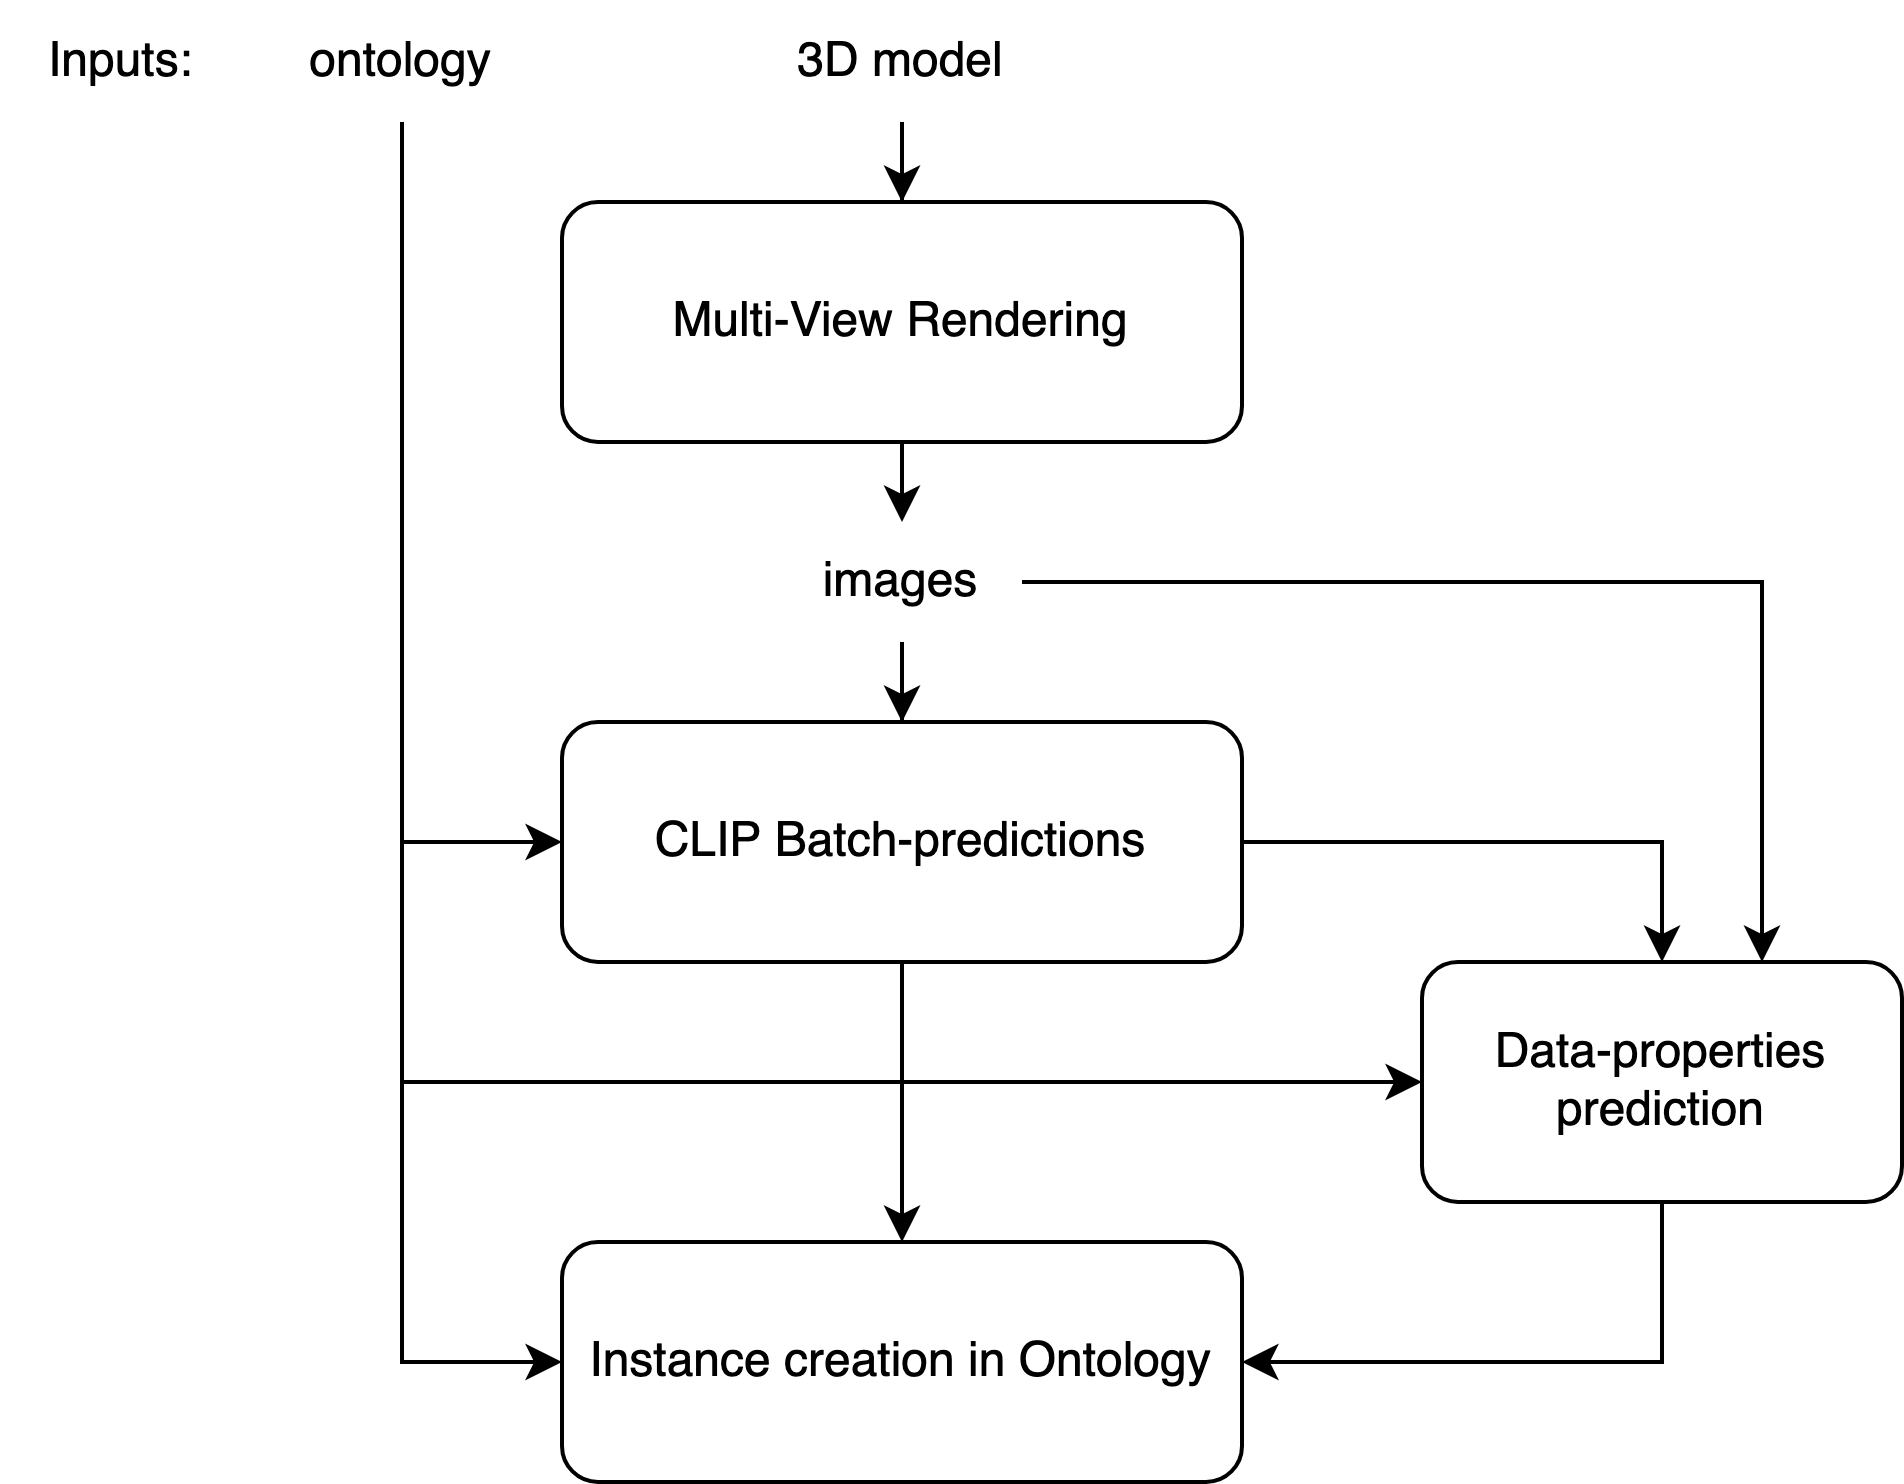
\includegraphics[width=0.6\textwidth]{figures/process}
  	\caption{Overview of the whole process}
  	
  	\label{fig:process}
  \end{figure}
  
  \subsection{Creating the Ontology}
  
  We started the investigation by creating a simple ontology to represent the digital twin of transport infrastructure, we used Stanford's Protégé \cite{protege}, a software for developing and managing ontologies, to create the following ontology, see figure \ref{fig:ontology}.
  \begin{figure}[h]
    \centering
  	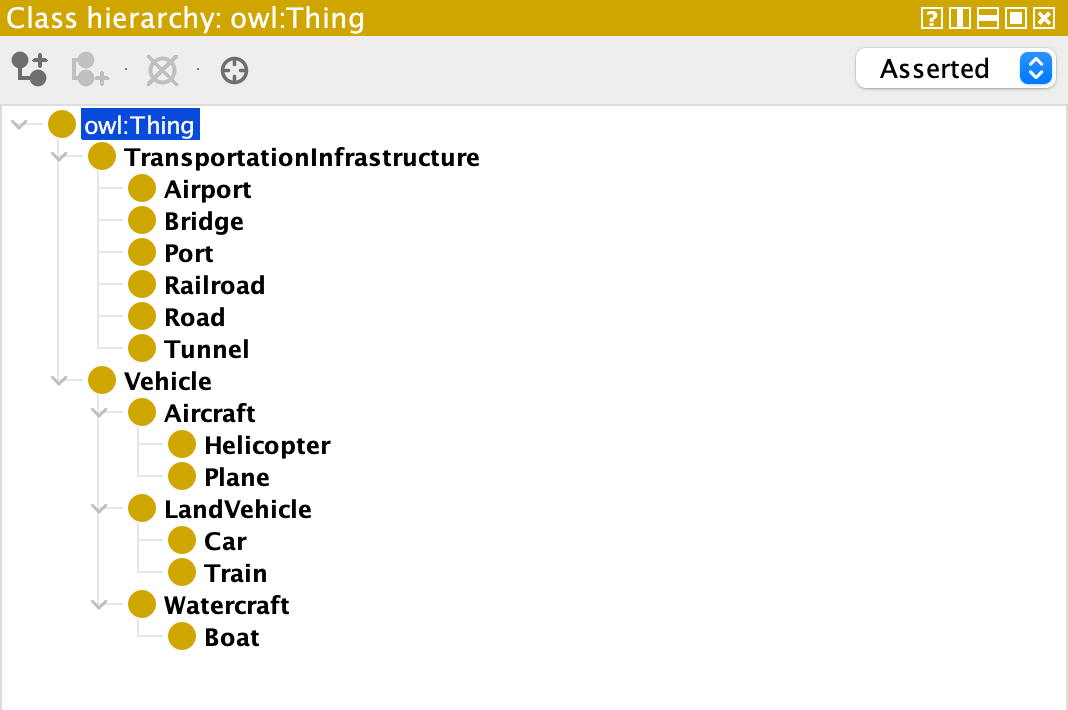
\includegraphics[width=0.6\textwidth]{figures/initial_ontology}
  	\caption{Simple Ontology}
  	\label{fig:ontology}
  \end{figure}
\\
  The ontology is in this case a simple taxonomy, meaning that the only relationship between the classes are \texttt{is-a} relationships or in this case \texttt{SubClassOf}. In this example, Plane is a subclass of Aircraft, then Aircraft is a subclass of Vehicle, and Vehicle is a sub-class of \texttt{owl:Thing}. Every class is implicitly a sub-class of \texttt{owl:Thing}, the later being the root of the ontology. OWL \cite{Bechhofer2009} stands for Web Ontology Language, it is a language used to describe ontologies in a format that can be shared in the web. Here in code snippet \ref{lst:ontologycode}, we can see how classes and relationships are defined with OWL in an XML (Extensible Markup Language) format, some details were omitted for brevity, see appendix for full code. The code was obtained by exporting the ontology as XML from Protégé.
  
  \begin{lstlisting}[language=XML, caption={OWL expressed in XML code for the ontology},label={lst:ontologycode}, mathescape=true, breaklines=true]
<?xml version="1.0"?>
<Ontology xmlns="http://www.w3.org/2002/07/owl#".../>
	<!-- How classes are declared -->
    <Declaration> 
        <Class IRI="Aircraft"/>
    </Declaration>
    <Declaration>
        <Class IRI="Vehicle"/>
    </Declaration>
    ...
    <!-- How relationships are defined -->
    <SubClassOf>
        <Class IRI="Aircraft"/>
        <Class IRI="Vehicle"/>
    </SubClassOf>
    ...
    <!-- defining disjoint classes e.g: an aircraft cannot be a watercraft or a land vehicle, a vehicle cannot be a transport infrastructure ... -->
    <DisjointClasses>
        <Class IRI="Aircraft"/>
        <Class IRI="LandVehicle"/>
        <Class IRI="Watercraft"/>
    </DisjointClasses>
    <DisjointClasses>
        <Class IRI="TransportationInfrastructure"/>
        <Class IRI="Vehicle"/>
    </DisjointClasses>
    ...
</Ontology>
  \end{lstlisting}
  This simple ontology will serve as the basis for classification as the model will predict based on the classes defined in the ontology. The naming we chose for the classes is no coincidence, in the next section, we will see why it is important to have expressive class names.
  
  \subsection{Classifying Images Based on Ontology Classes}
  In order to make the process independent of any dataset or ontology, we had the idea of using a zero-shot classifier. Zero-shot classifiers can predict classes which they have never seen before, it is a type of transfer learning. The concept is mostly prevalent in natural language processing (NLP), a model is presented with a prompt and a list of classes (some of which the model has never seen before), then the model predicts to which class the prompt belongs. Ideally, we would give the zero-shot classifier an image and a list of possible classes, and it should be able to predict the probabilities of the image belonging to any of the given classes. OpenAI's open-source CLIP \cite{radford2021learning}(Contrastive Language-Image Pre-Training) model does just that, it is a multi-modal model that is able to classify an image based on a given set of classes. The most interesting part is that it can classify also for classes it has never seen before, it is hence a zero-shot classification model. Before explaining how the model works in more detail, it is best to show an example. Code snippet \ref{lst:clipcode} shows how the model can be used.
  
  \begin{lstlisting}[language=Python, caption={Using CLIP model},label={lst:clipcode}, mathescape=true, breaklines=true]
# inputs
image_path = './images/porsche.jpg'
classes = ['car', 'boat', 'plane']
  	
# using the model
model = CLIPModel.from_pretrained("openai/clip-vit-large-patch14")
processor = CLIPProcessor.from_pretrained("openai/clip-vit-large-patch14")
inputs = processor(text=classes, images=Image.open(image_path), return_tensors="pt", padding=True)
outputs = model(**inputs)
logits_per_image = outputs.logits_per_image 
probs = logits_per_image.softmax(dim=1).cpu().detach().numpy() 
# outputs
list_probs = probs[0].tolist()
#### result:
car: 0.9976612329483032
boat: 0.001253269612789154
plane: 0.0010854981373995543
  \end{lstlisting}
  
  The code for snippet \ref{lst:clipcode} was obtained from the CLIP documentation made by Hugging Face \cite{huggingfaceCLIP}. As you can see, we gave the model as input an image of car as JPG file and a list of classes and the model gave the correct prediction, which is class "car". The researchers behind CLIP suggest feeding the classes as "\texttt{a photo of a \{className\}}" for better predictions, the reason for this will be explained in the next section. CLIP was in fact used by OpenAI to evaluate their DALL·E \cite{dall-e} model's performance.
  \subsubsection{How CLIP works}
  CLIP was trained on 400 million image-text pairs. A general overview of how CLIP works can be seen in figure \ref{fig:clip_overview}, it was taken from the original CLIP paper \cite{radford2021learning}.
  \begin{figure}[h]
  	\centering
  	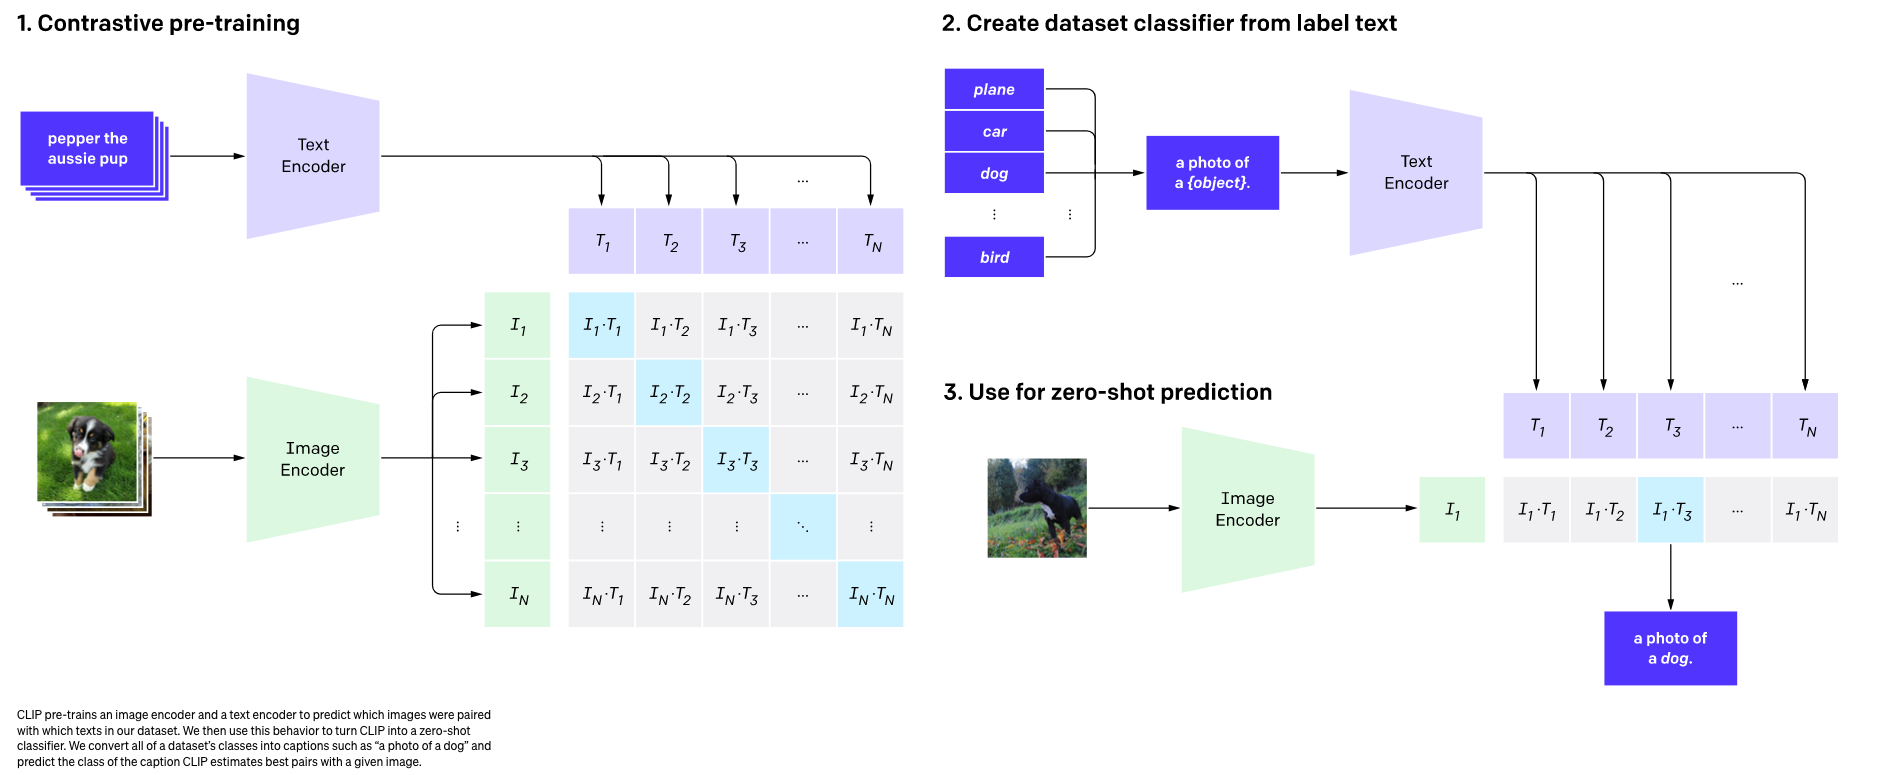
\includegraphics[width=\textwidth]{figures/clip_overview.png}
  	\caption{CLIP Overview \cite{radford2021learning}}
  	\label{fig:clip_overview}
  \end{figure}
  \\
  \textbf{1. Contrastive pre-training:}
  \\
  The first step is training the model. That means training the image encoder and the text encoder at the same time. To do so, a list of images $Img$ and their respective textual descriptions $Txt$ are used, i.e $Txt_i$ is the textual description of $Img_i$. The images are fed into an image encoder that computes the image vector $I$, and the same thing is done with the texts using a text encoder where we compute the text vector $T$. Where $I_i$ is the generated vector representation of $Img_i$ and $T_i$ is the generated vector representation of $Txt_i$. The image encoder is a slightly modified version of the Vision Transformer (ViT) described in the paper titled "An Image is Worth 16x16 Words" \cite{dosovitskiy2021image} which managed to overcome the token limit imposed by the self-attention mechanism associated with traditional transformers \cite{vaswani2017attention}, while the latter works very well for text in the context of NLP, it doesn't scale to images, since in keeping with the self-attention mechanism, each pixel would need to attend to every other pixel for calculating the pair-wise inner product. The quadratic cost would therefore not scale to the huge number of pixels that an image typically contains, resulting in very expensive computations. ViT avoids this issue by splitting the image into fixed-size patches, then the patches are multiplied by a learnable weight matrix to further reduce the dimensions of the patch, this multiplication process is known as linear mapping. This transforms the image into a format that the traditional transformer encoder can support. The resulting vectors are then fed as tokens to the encoder and it is this output that CLIP will use in the subsequent steps. As for the text encoder, they used the transformer described in \cite{Radford2019} (the GPT-2 paper). Afterwards, the two transformers are trained in a very special way, instead of being trained separately, they always consider the modality of each other. That is done by maximizing the dot products $I_i\cdot T_i$ and minimizing $I_i\cdot T_j \: where \: i \neq j$, this is known as contrastive training, where the model will not only learn how to associate but also learn to differentiate. 
  \\ \\
  \textbf{2. Zero-shot prediction:}
  \\
  After the training is done, it is now time for predictions. To run a zero-shot prediction on a list of classes, some prompt engineering is in order, instead of simply using the class name, we should instead use "a photo of class\_name". This is due to the fact that CLIP was trained on image-text pairs that were scrapped from the web and notably from social media posts, so the text is usually a description of the contents of the image, using the "a photo of " prefix lets us specify to CLIP that we are interested in the content of the image, in fact, the CLIP paper mentions that there is a 1\% accuracy improvement when using "a photo of class\_name". After applying the prefix to our list of strings, the next step is to compute the text vectors $T_i$ for each of the classes using the trained text transformer and to compute the image vector $I_1$ using the trained Vision Transformer, we then calculate the inner products $I_1 \cdot T_i$, the biggest inner product is taken as the result of the prediction.
  \subsubsection{Using CLIP to classify an image with ontology classes}
  To use CLIP with ontology classes, we had the idea of traversing the ontology as a tree. At first, the children classes of the root class \texttt{owl:Thing} will be taken as input classes, then we run CLIP on these classes with the input image. The class with the highest probability is then chosen and its children classes are used as input classes and the zero-shot predictions are run on those children classes. The process repeats itself again until we reach a leaf. The leaf is then considered the predicted class. See algorithm \ref{alg:ImgOntoClassification} for the pseudo-code. (Note: Actual python implementations differs slightly from the pseudo-code due to how the ontology library (owlready2 \cite{owlready2}) we used works)
  	\begin{algorithm}
  		\caption{Ontology Based Image Classification with CLIP}\label{alg:ImgOntoClassification}
  		\begin{algorithmic}
  			\Function{Classify}{$image, ontology$}
  			\State $currentClasses \gets \Call{getRootClasses}{ontology}$
  			\State $currentProbabilities \gets \Call{CLIPPredict}{currentClasses, image}$
  			\State $maxIndex \gets$ index of maximum value in $currentProbabilities$
  			\State $chosenClass \gets currentClasses[maxIndex]$
  			\While{$chosenClass$ is not a leaf}
  				\State $currentClasses \gets \Call{getChildren}{chosenClass}$
  				\State $currentProbabilities \gets \Call{CLIPPredict}{currentClasses, image}$
  				\State $maxIndex \gets$ index of maximum value in $currentProbabilities$
  				\State $chosenClass \gets currentClasses[maxIndex]$
  				\State $chosenProb \gets currentProbabilities[maxIndex]$
  			\EndWhile
  			
  			\State \Return $chosenClass, chosenProb$
  			\EndFunction
  		\end{algorithmic}
  	\end{algorithm}
  	
  	\subsection{Creating a 3D renderer}
  	Now that we have it figured out for how to classify an image using ontology classes, the next step is to turn the 3D model into a 2D image that can be fed to the above mentioned algorithm. Previous research demonstrated that using a multi-view representation (rendering the 3D object from multiple view points)  yielded far more efficient results than using a descriptor or the raw 3D mesh, see the literature review section for more detail. On our side, we opted for multi-view representation where the number of images to render can be specified, we chose to keep this number low since we noticed that running algorithm \ref{alg:ImgOntoClassification} can get very expensive when using too many pictures without any clear improvements in terms of accuracy compared to using fewer picture. Figure \ref{fig:multicarp5} shows what multi-view rendering is, the red points are cameras pointing at the object and the object is in the middle of the sphere (the figure was generated using p5.js \cite{p5js}). 
  	\begin{figure}[h]
  	\centering
  	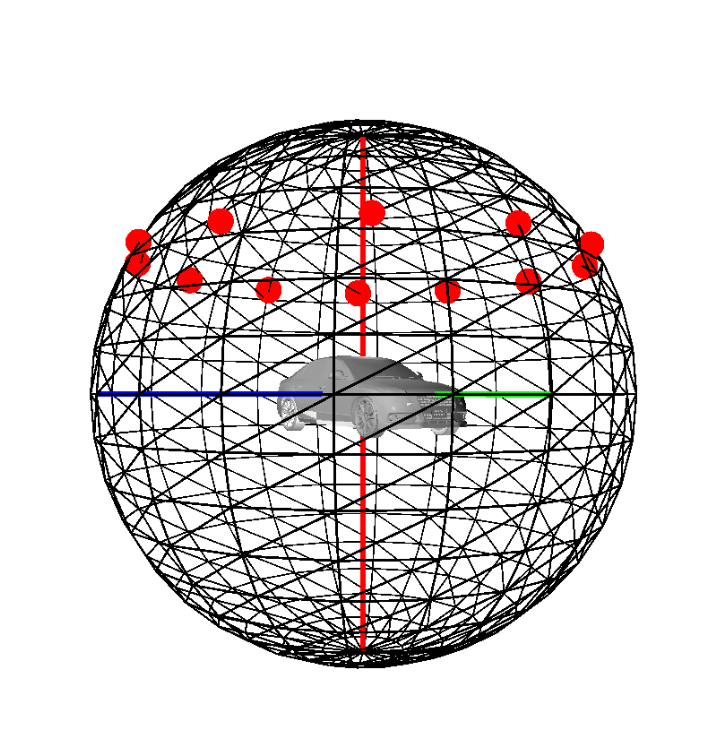
\includegraphics[width=0.6\textwidth]{figures/multiviewcar.png}
  	\caption{Multi-view rendering}
  	\label{fig:multicarp5}
  \end{figure}
  \subsubsection{Calculating the bounding sphere}
  Given the large size variety of 3D objects, the cameras must be placed sufficiently away in order to get the full object in frame. To do so, we calculate the bounding sphere then multiply its radius by a factor then use it as the camera distance. The bounding sphere should contain all of the vertices of the 3D object. There are a variety of algorithms out there to compute a bounding sphere. Some like Ritter's algorithm \cite{ritter} calculate an approximation of the bounding sphere. We opted for a naive algorithm that calculates the exact bounding sphere, we used NumPy \cite{harris2020array} to do so in two lines of code. The first step is to calculate the center of the 3D object, which is also the center of the bounding sphere, by calculating the mean over numpy axis zero, so from top to bottom for each axis. This will yield a 3D point which will be the center of the bounding sphere, see line 3 in listing \ref{lst:center}, it will also be used in the next step to compute the radius of the sphere.
 \begin{lstlisting}[language=Python, caption={Calculating the bounding sphere},label={lst:center}, mathescape=true, breaklines=true]
import numpy as np
verts = verts.numpy()              # convert vertices into numpy format
center = np.mean(verts, axis=0)    # calculate the center 
radius = np.max(np.linalg.norm(verts - center, axis=1)) # the radius
\end{lstlisting}
 To compute the radius, we have to first calculate the distances between each vertex and the center of the sphere.
 $$dist(v_i - c_{sphere}) = \| v_i - c_{sphere} \|$$ 
 We then take the maximum of these distances and that should give the largest distance between a vertex and the center, which turns out to be the radius of the sphere, see line 4 of in listing \ref{lst:center} for Numpy implementation. 
 $$r_{sphere} = max(dist(v_1 - c_{sphere}), dist(v_2 - c_{sphere}), \cdots, dist(v_n - c_{sphere}))$$ 
 \subsubsection{Multi-view rendering}
 Before describing the rendering process, we have to first specify which type of 3D file we will be using. We opted for the Wavefront \texttt{.obj} \cite{obj} file format since it is the most widely-used format and very lightweight, it is also very easy to read and write. While the \texttt{.obj} file defines the geometry of the 3D object, it also references a \texttt{.mtl} file which describes the materials and which by its turn usually references texture files (\texttt{.jpg}, \texttt{.png}, \texttt{.bmp} ...). Since we wanted to keep the whole process in one programming language, we used the PyTorch3D python library \cite{ravi2020pytorch3d} for rendering.  To make the renderer, we used PyTorch3D's guide as well as this tutorial \cite{mediumPyTorch3D}. Before explaining how multi-view rendering is done with PyTorch3D, let's first explain what parameters the render process takes. The multi-view rendering pipeline is very customizable, it is defined as follows:
\\ \\
\textbf{Arguments:}
\begin{itemize}
  \item \verb|obj_filename: file path of the .obj file to be rendered|
  \item \verb|camera_dist : camera distance from the 3D model|
  \item \verb|elevation   : camera elevation (default=30)|
  \item \verb|image_size  : size of the output image in pixels|
  \item \verb|batch_size  : number of images to render|
\end{itemize}
\textbf{Output:}
\begin{itemize}
  \item \verb|images      : list of images of length=batch_size|
\end{itemize}

\verb|elevation| is set to a default of 30 in order to get somewhat of an aerial view of the object, it refers to the angle between the horizontal plane $xz$ and the vector between the camera and the object center, see Figure \ref{fig:distelev}. As for \verb|camera_dist|, its value is determined by the previously calculate bounding sphere radius multiplied by a factor of $2.5$. The factor was chosen after trial and error. The first step is to load the 3D object into a mesh object that PyTorch3D can handle. Afterwards, the cameras are defined. The elevation and camera distance are the same for all cameras, except the azimuth angle which rotates the camera around the $y$ axis which goes through the center of the object, see Figure \ref{fig:azim}. The batch size is used to determine to set the different azimuth angles, that is done with \verb|torch.linspace(0, 330, batch_size)|. Which will generate a 1D tensor of size \texttt{batch\_size} that contains evenly spaced values between \ang{0} and \ang{330} which means a full circle around the object. Afterwards we define the rasterizer, its task is to project the 3D scene into the camera's 2D viewing plane and generate a 2D image, so this is where the image dimensions are specified using the initially given \texttt{image\_size}. As for the shader, a Phong shader \cite{phong} is used. Then the renderer is defined by combining the rasterizer and shader, and the images are finally rendered. See Figure \ref{fig:carrender} for a car 3D model that I rendered using \verb|batch_size=12|.

\begin{figure}[H]
     \centering
     \begin{subfigure}{0.5\textwidth}
         \centering
         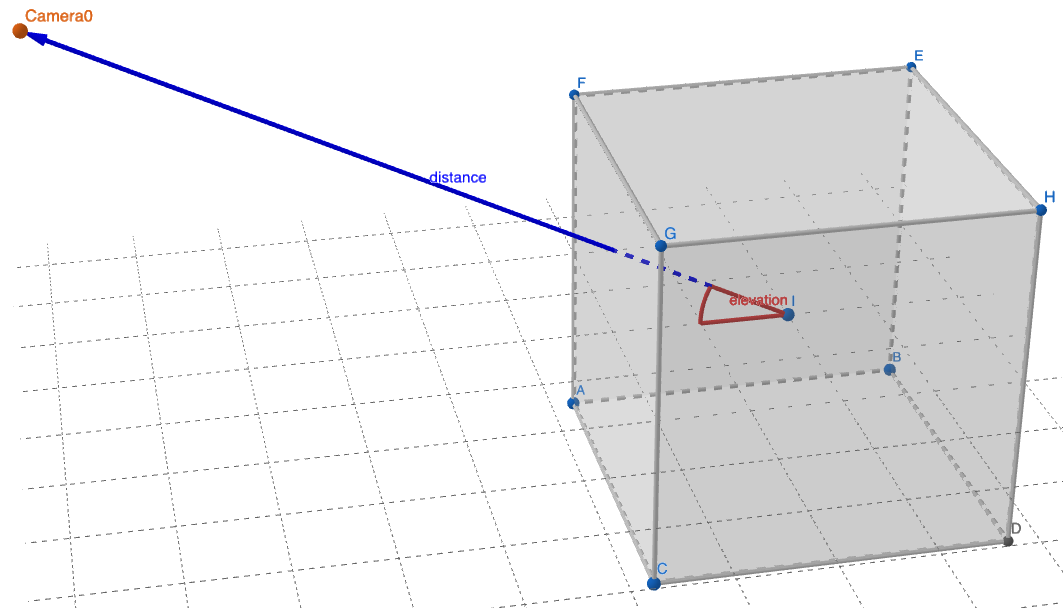
\includegraphics[width=\textwidth]{figures/multi1.png}
         \caption{}
         \label{fig:distelev}
     \end{subfigure}
     \hspace*{\fill}
     \begin{subfigure}{0.4\textwidth}
         \centering
         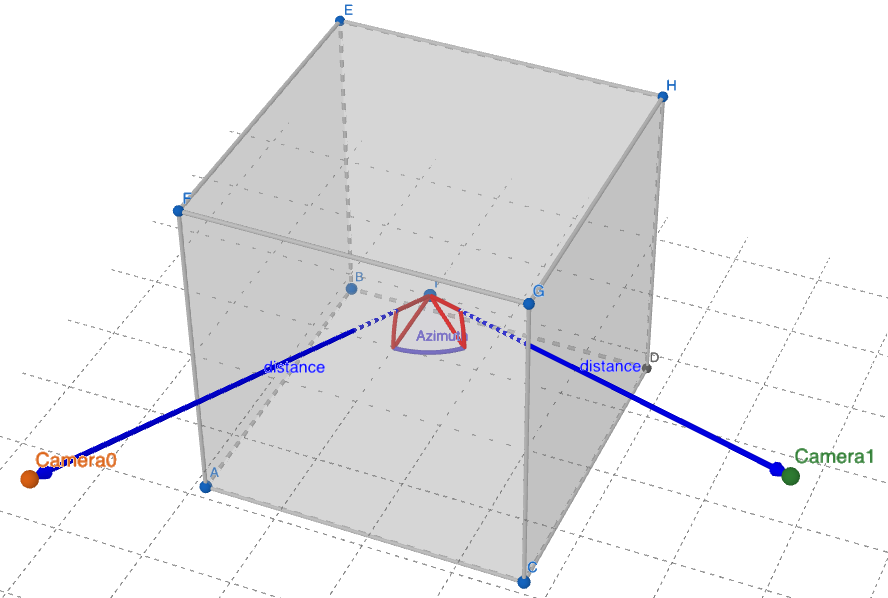
\includegraphics[width=\textwidth]{figures/multi2.png}
         \caption{}
         \label{fig:azim}
     \end{subfigure}
        \caption{}
        \label{fig:two}
\end{figure}
\begin{figure}[h]
  	\centering
  	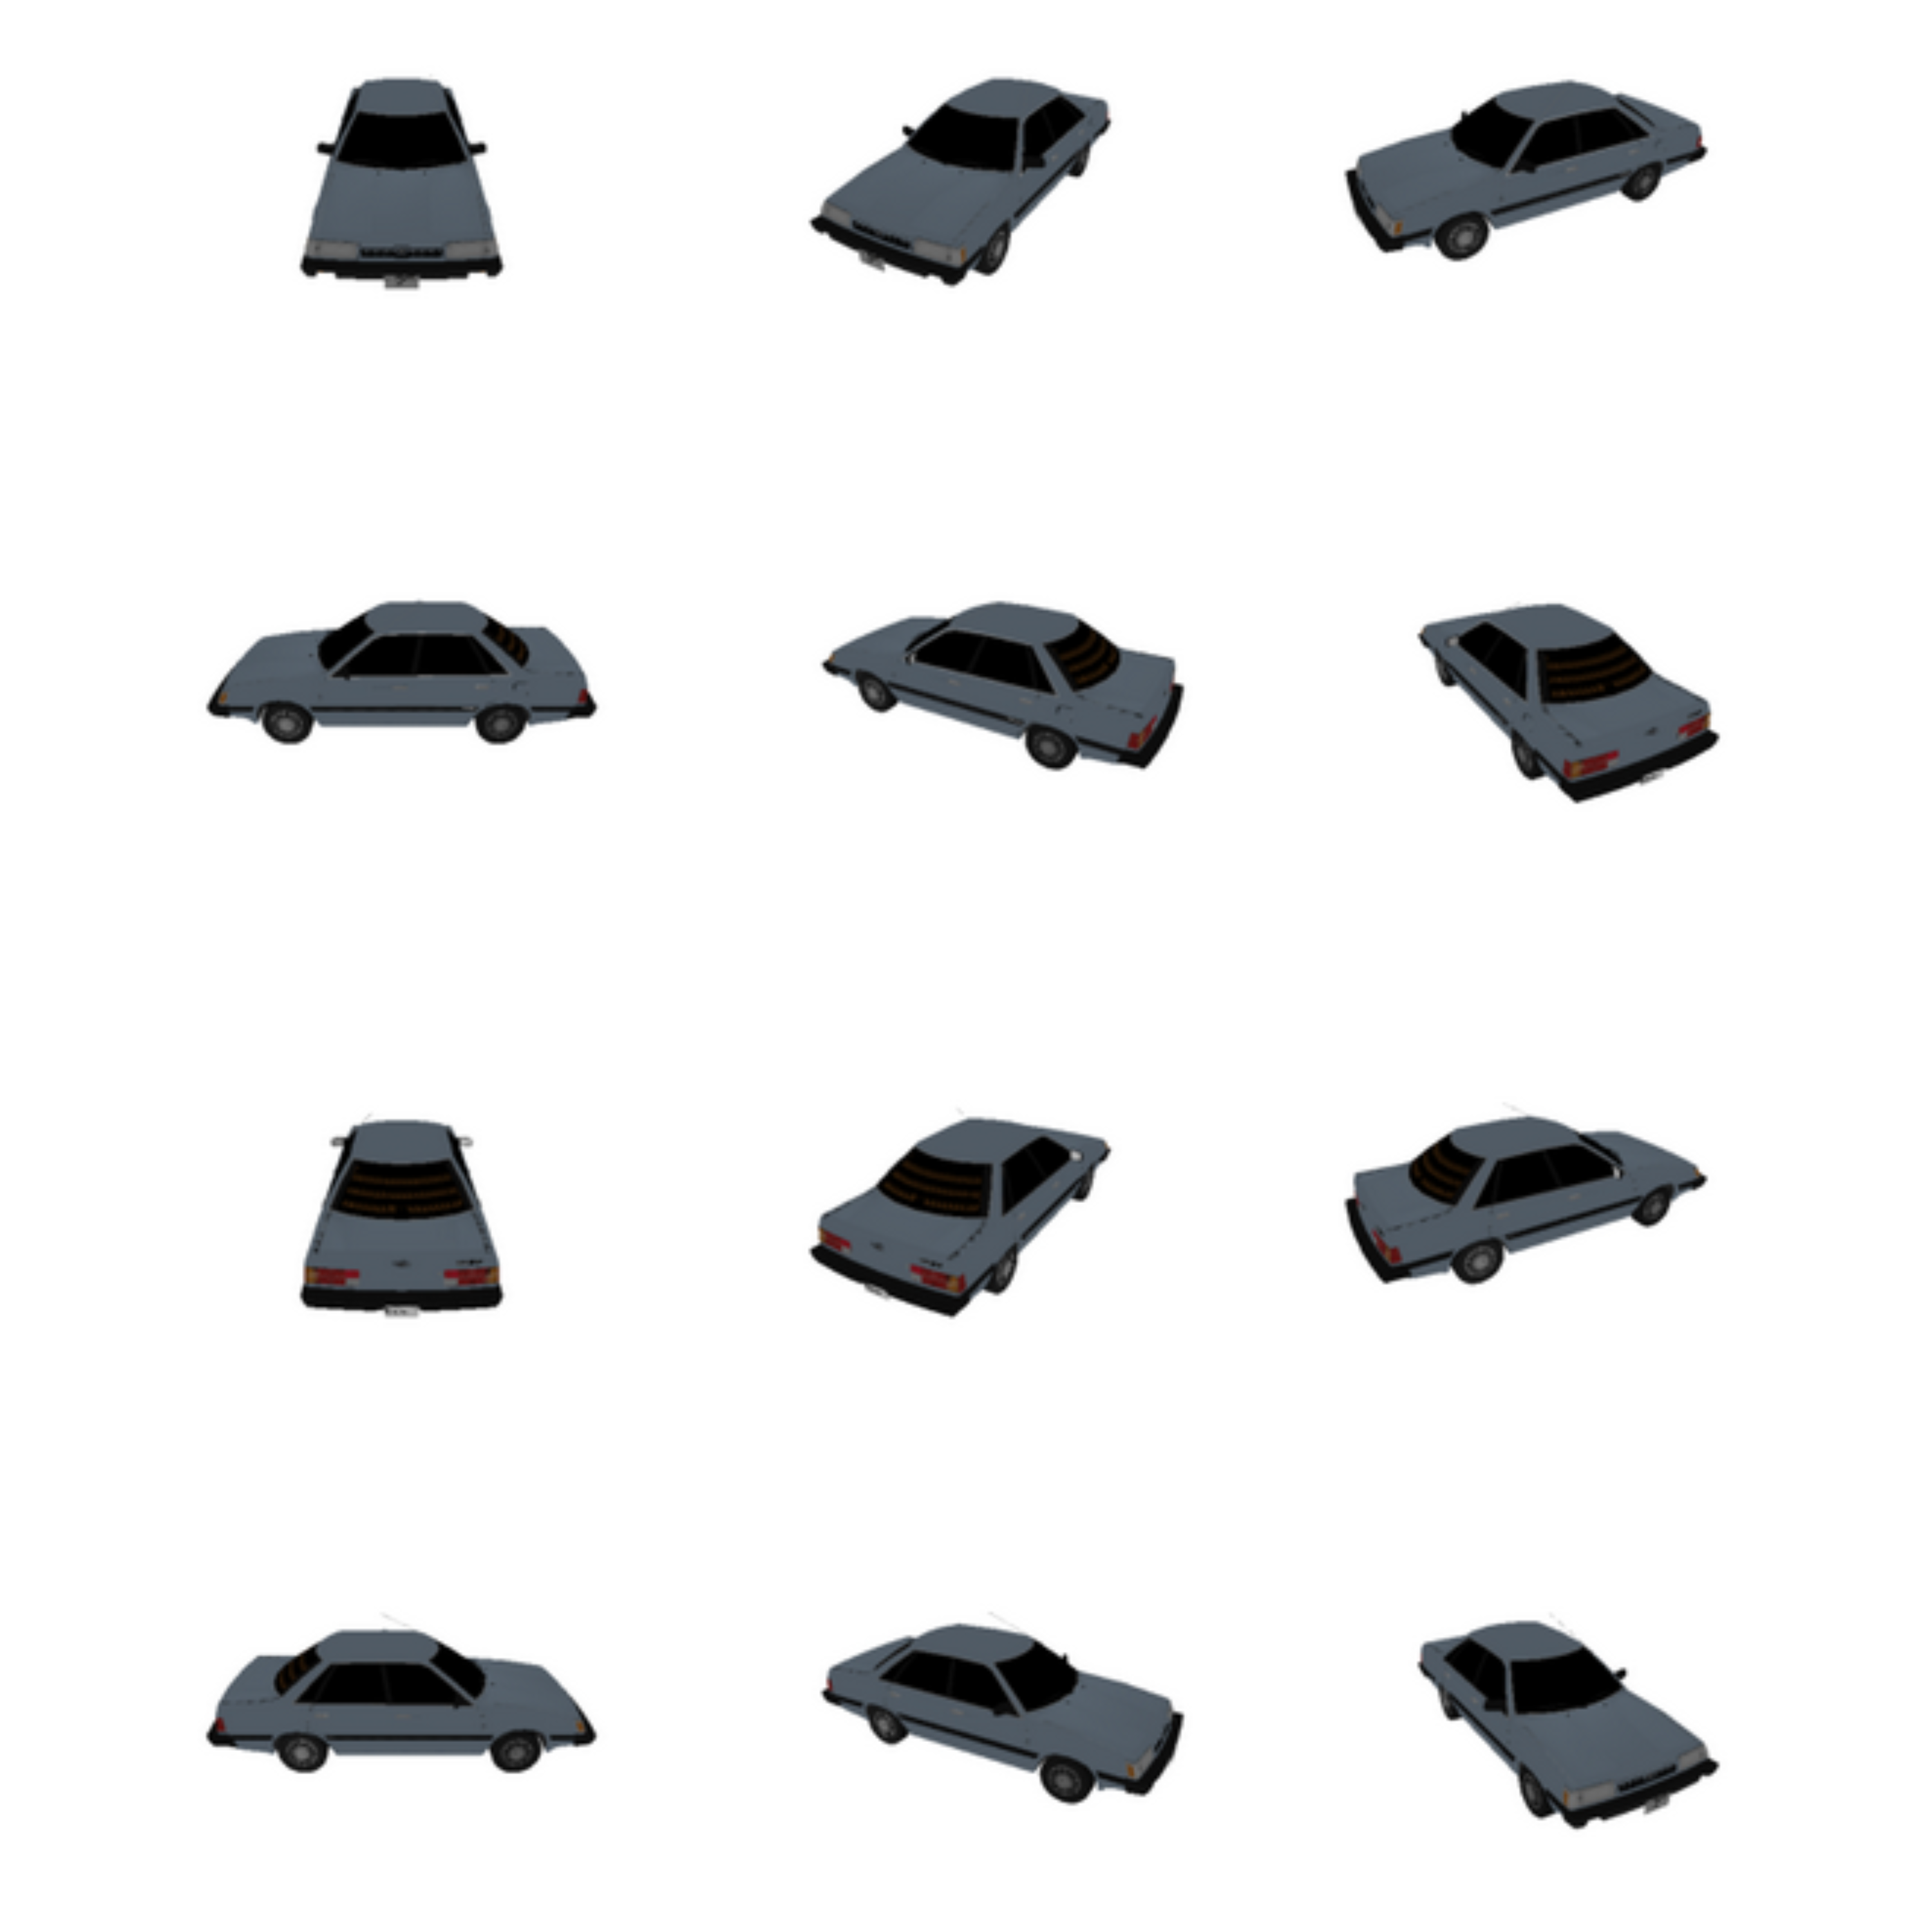
\includegraphics[width=0.4\textwidth]{figures/render_car.png}
  	\caption{Rendered images of a car 3D model}
  	\label{fig:carrender}
\end{figure}
\subsection{3D Object CLIP zero-shot classification with ontologies}
In order to adapt 2D image classification to 3D models, the images rendered from the previous section are used with the previously developed image classification on ontologies process (Algorithm \ref{alg:ImgOntoClassification}). To do so, we loop over all the generated images and run the classification on each one of them. The result is a list of key-value pairs where the key is the class and the value is the prediction. The next problem that arises is how we can determine only one entry from this list of key-value pairs to be the actual result of the predictions. Since there is room for error, some classifications may be false. A solution is to simply sum up the probabilities associated with each class and the class with the highest sum will be chosen as the predicted class. This approach manages to take into account both the occurrence of the class as well as the associated probability of each class. It is better than taking the averages of each class since by taking the average we can obtain a smaller value if the class occurs many times and a bigger value if the class appears only once, hence undermining the importance of the number of occurrences of a class. See Algorithm \ref{alg:3DOntoClassification}.
\begin{algorithm}[H]
  		\caption{Ontology Based 3D model Classification with CLIP}\label{alg:3DOntoClassification}
  		\begin{algorithmic}
  			\Function{Classify3D}{$object, ontology, batch\_size, image\_size$}
  			\State $predictions = \emptyset$
  			\State $radius \gets \Call{boundingSphereRadius}{object}$
  			
  			\State $images$ $\leftarrow$ \Call{BatchRender}{$object$,  $camera\_dist=radius*2.5$, $image\_size$, \hspace*{2.3\mylen}$batch\_size$} 
  			\ForEach {$image \in images$}
  				\State $class, prob \gets \Call{Classify}{image, ontology}$
  				\State $predictions \cup (class, prob)$
  			\EndFor
  			\State $chosenClass \gets class$ with maximum sum of $prob$ in $predictions$
  			\State \Return $chosenClass$
  			\EndFunction
  		\end{algorithmic}
\end{algorithm}
\subsection{3D Object CLIP zero-shot classification with ontology data properties }

We managed to use CLIP in order to classify the data property of a class. In our example, we created a color data property for the Vehicle class which is of data type string. To then predict this data property using CLIP, we had to do some prompt engineering. In the case of this data property, we used the prompt "a photo of a '\texttt{color}' '\texttt{vehicle}'". The possibilities for the data property must be stored as a json array in the metadata of the data property, it is crucial that all the possibilities must be known, so for the color property, a JSON array containing different colors is used. The data property must also be a visual feature of the object to predict. see \texttt{predict\_Vehicle\_data\_properties} in \texttt{functions.py}

\subsection{Integrating the detected 3D object into the ontology}
As a final step, the object must be integrated into the ontology. To do so, an individual is created for the predicted class. For further completeness, the metadata of this individual stores information such as the creation date and the file path of the original \texttt{.obj} file. Then we check if the class has any data properties, if so, these are also accordingly set using CLIP. As for the naming convention of these created instances, we use the class name suffixed with an index. See \texttt{createInstance} in \texttt{functions.py}

\section{Evaluation of the Investigation}
  
  \subsection{Tools Used}
  Since the whole process was written in Python, we used Jupyter Notebook \cite{Kluyver2016jupyter} to carry out the tests (see \texttt{Validation.ipynb}). We used Pandas dataframes \cite{mckinney-proc-scipy-2010} to store the result in csv format and matplotlib \cite{Hunter:2007} to make the graphs. For the rendering we used PyTorch3D \cite{ravi2020pytorch3d}.
  \subsection{Experiment Setup}
  To evaluate the whole process, we tested it with some models from popular 3D models repositories, mainly CG Trader \cite{cgtrader}. We used free models, some models were imported into Blender \cite{blender} then exported as OBJ. Some models are textured and some are not. The sizes of the models varies greatly as well. All the runs can be accessed in \texttt{runs.csv}. Please note that we used the CPU (M1 MacBook with 8GB RAM) for both rendering and running CLIP, that explains the higher run times. All the 3D models can be found in the \texttt{data} folder. See table 1 below.

  
\begin{table}[H]
\label{fig:3Dobjects}
\caption{Overview of used 3D models}
\centering
\begin{tabular}{|c|c|c|c|c}
\hline
\textbf{Class} & \textbf{\# Models} & \textbf{\# Textured} &  \textbf{Previews}\\
\hline
Car & 5 & 2 & 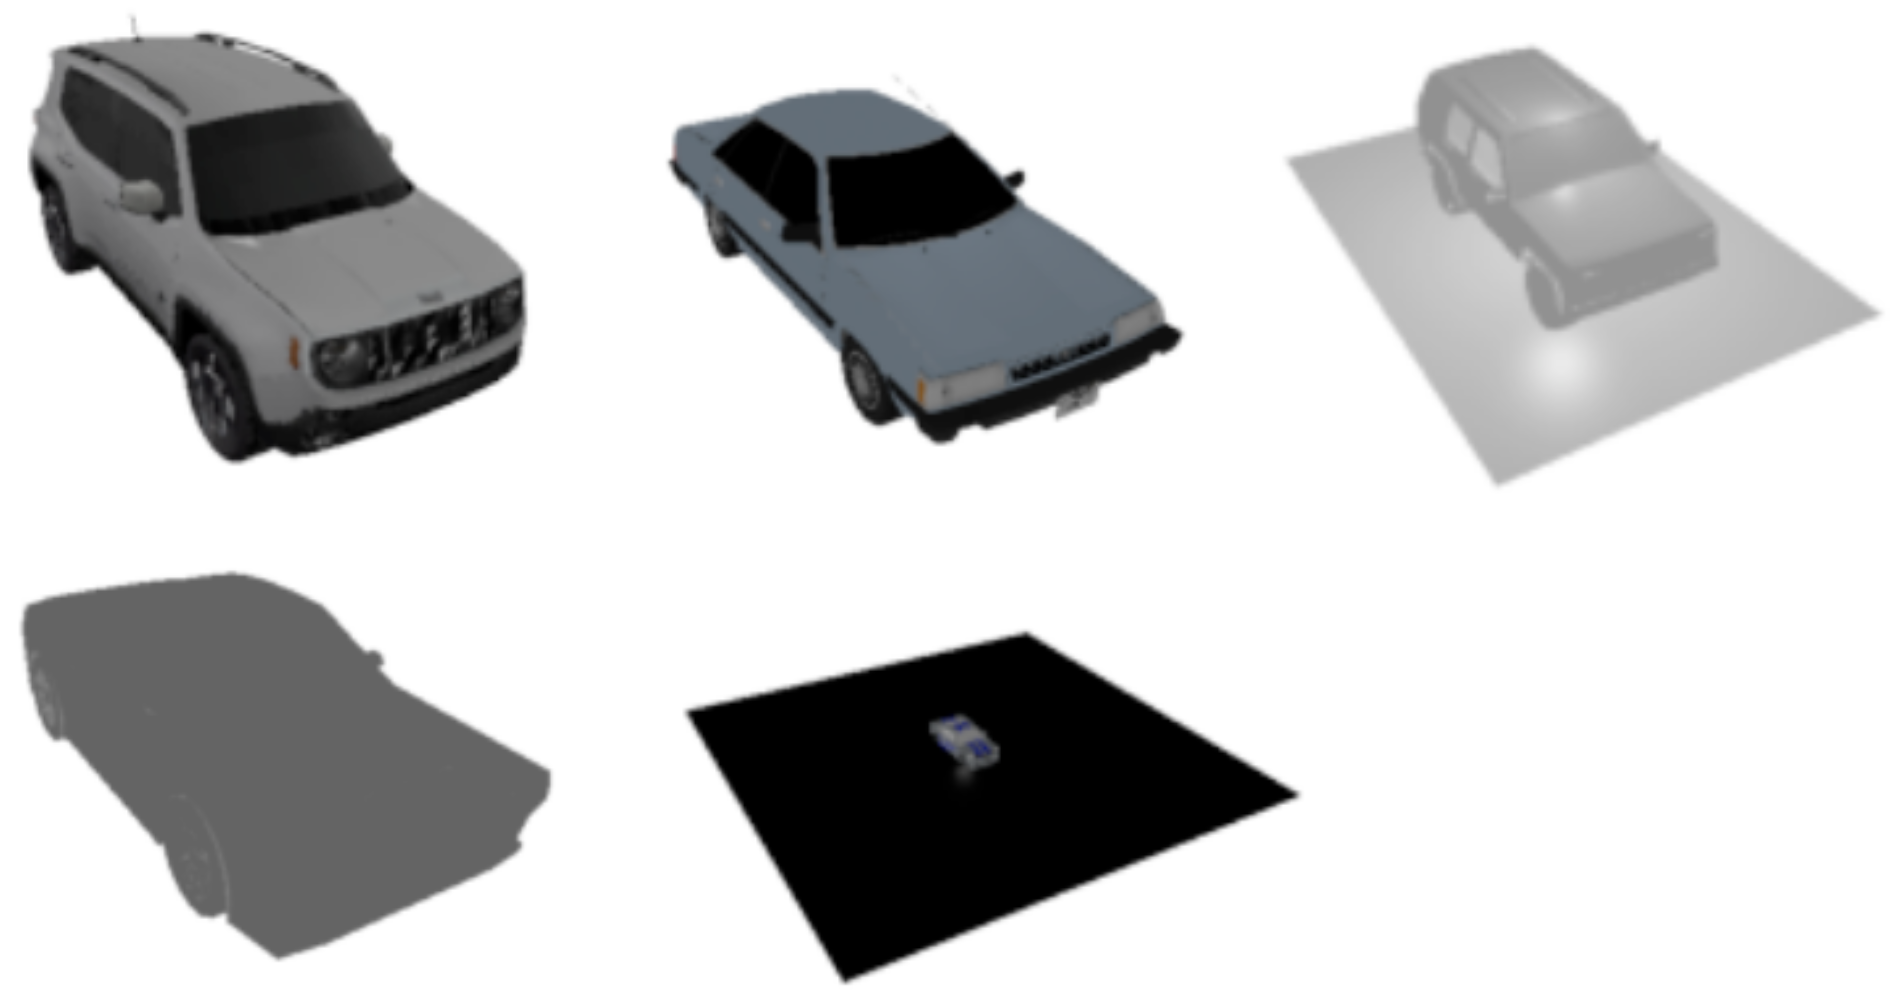
\includegraphics[width=4cm, height=3cm, keepaspectratio]{figures/cars.png}\\
\hline
Helicopter & 5 & 2 & 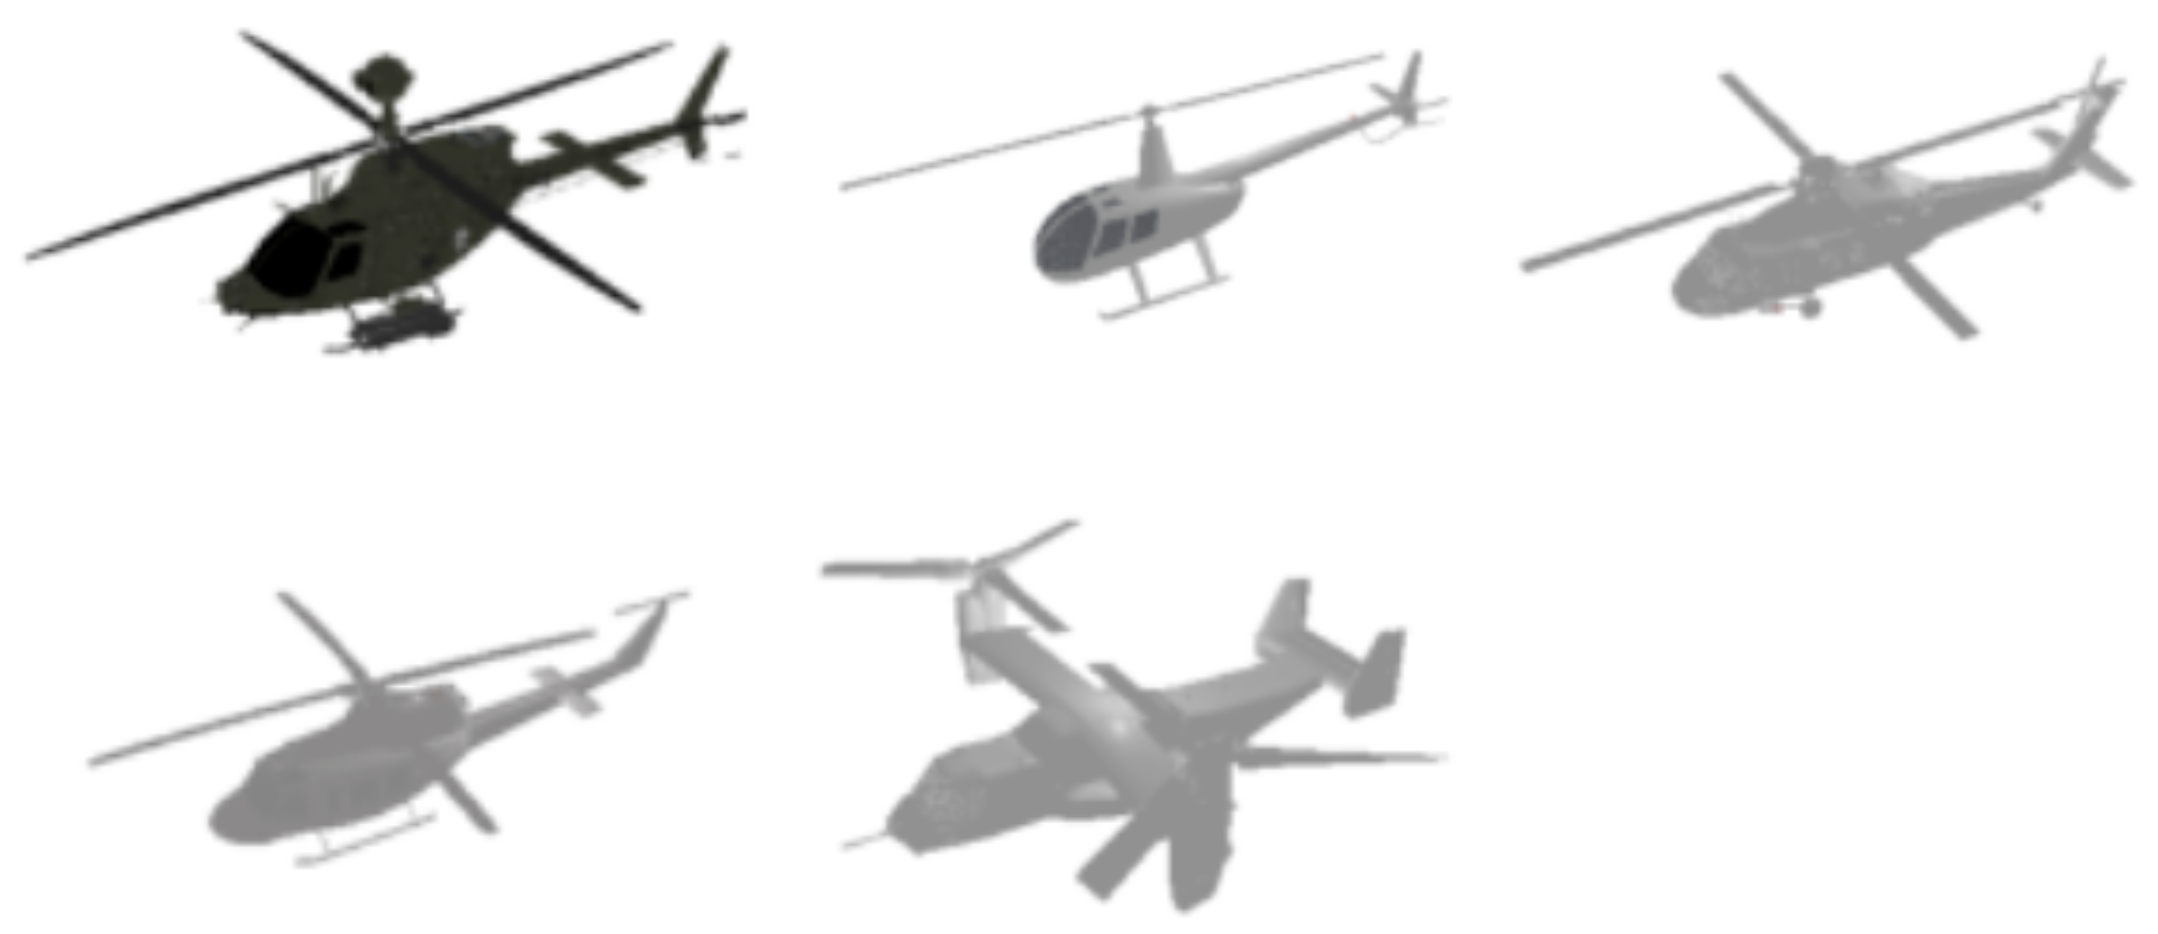
\includegraphics[width=4cm, height=3cm, keepaspectratio]{figures/helicopters.png}\\
\hline
Plane & 5 & 3 & 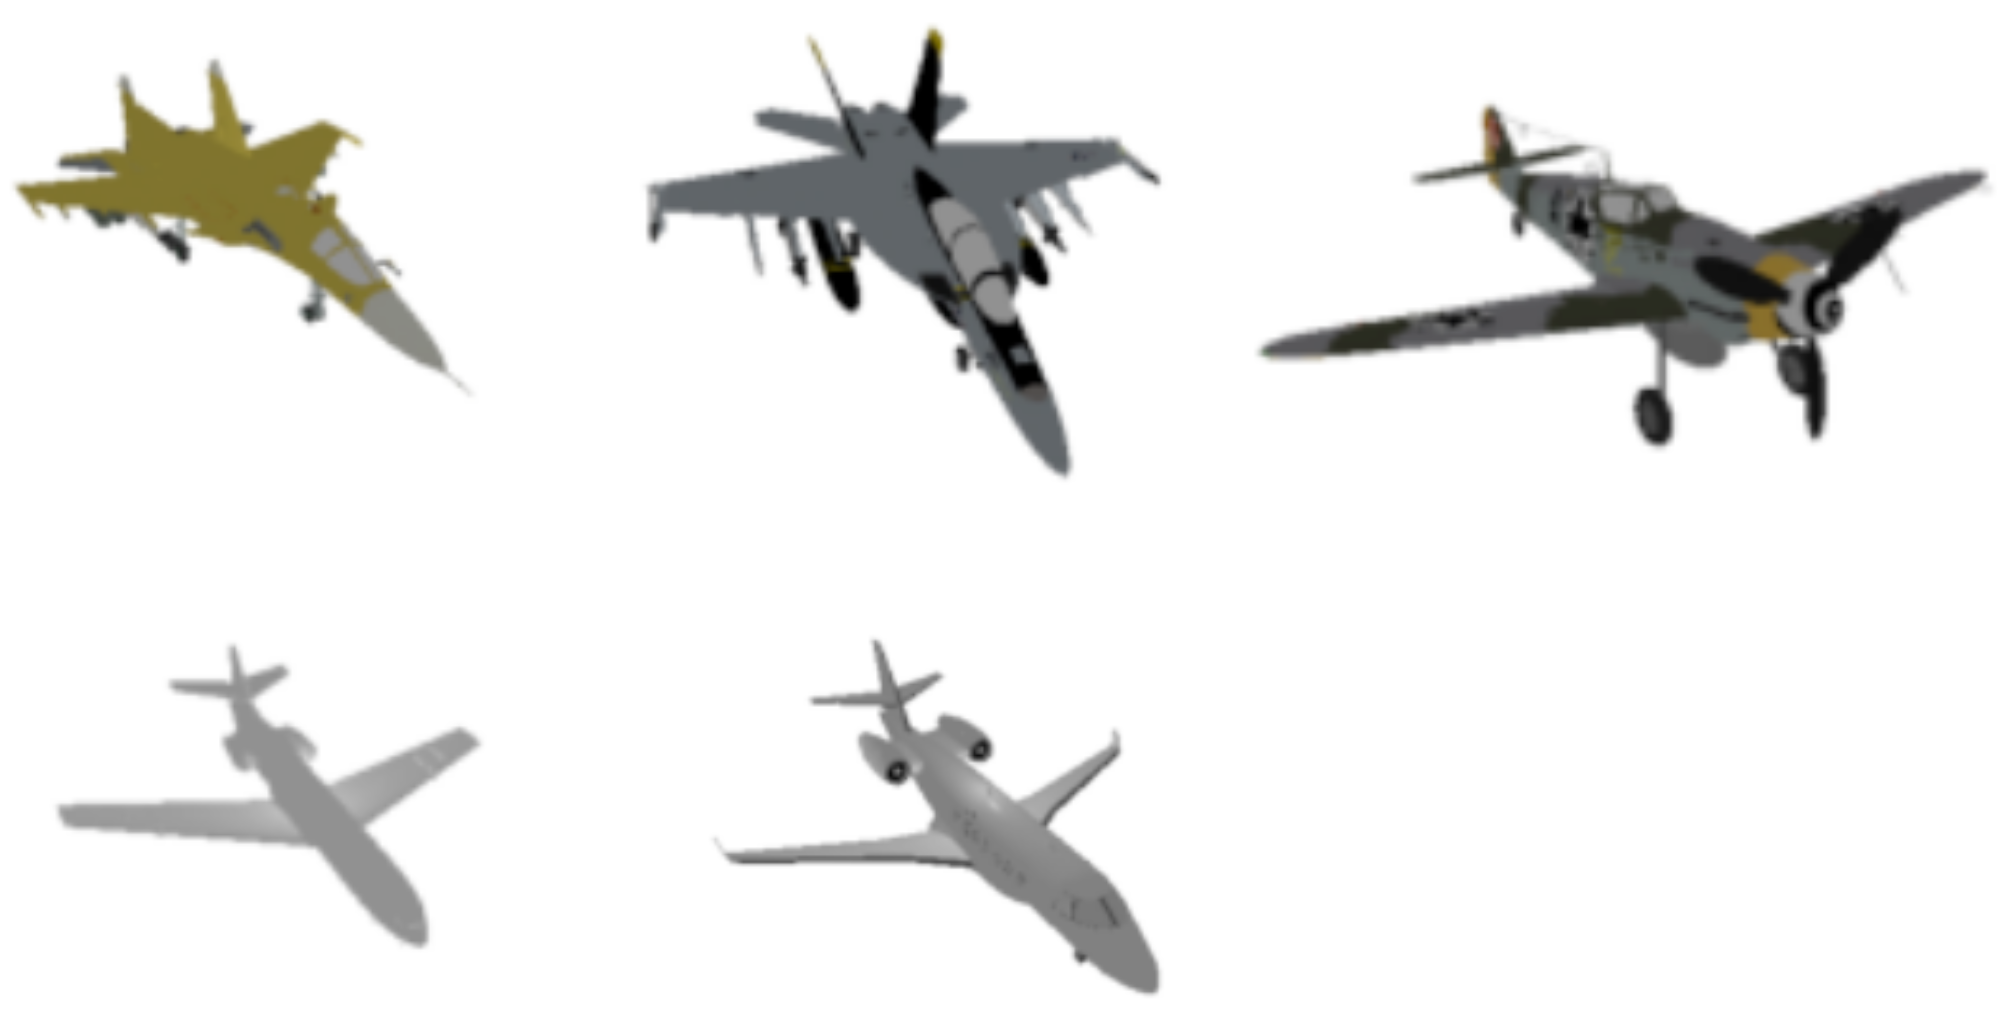
\includegraphics[width=4cm, height=3cm, keepaspectratio]{figures/planes.png}\\
\hline
Train & 5 & 3 & 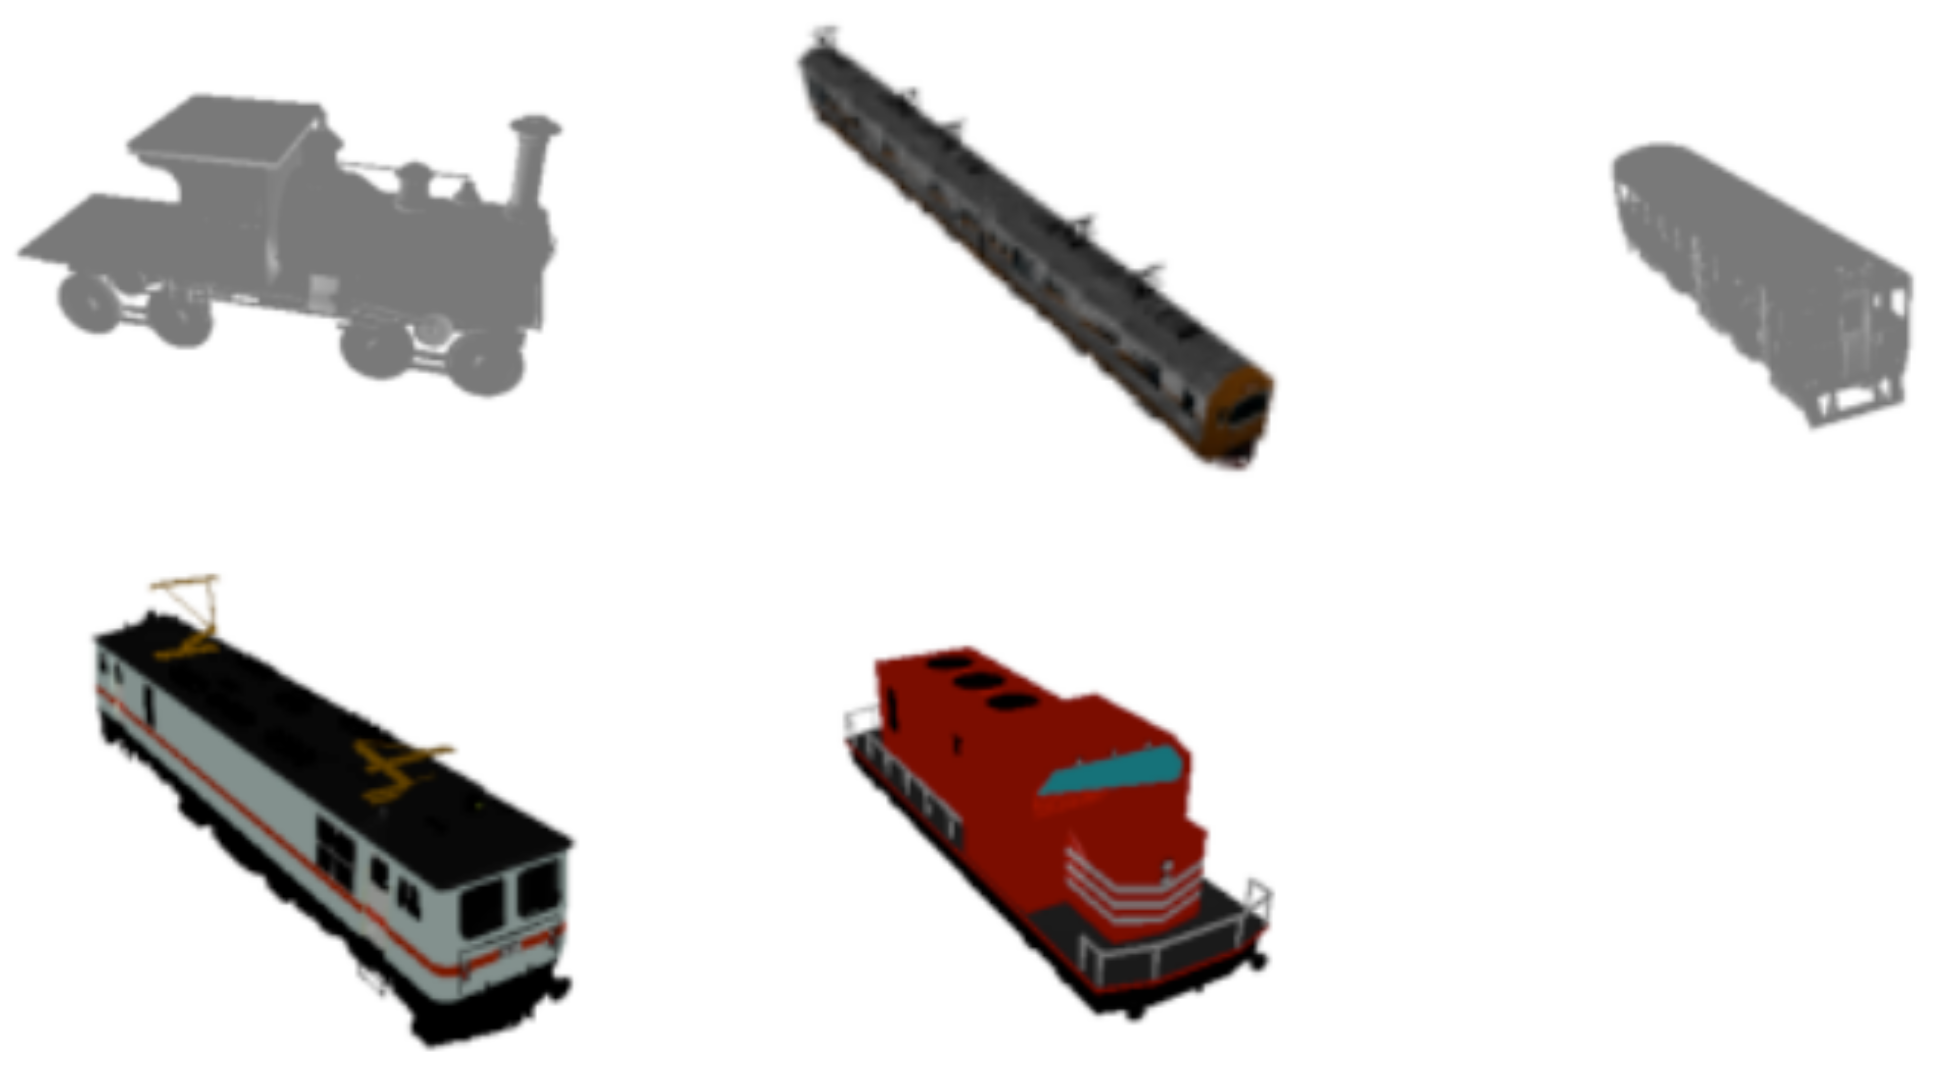
\includegraphics[width=4cm, height=3cm, keepaspectratio]{figures/trains.png}\\
\hline
Railroad & 1 & 0 & 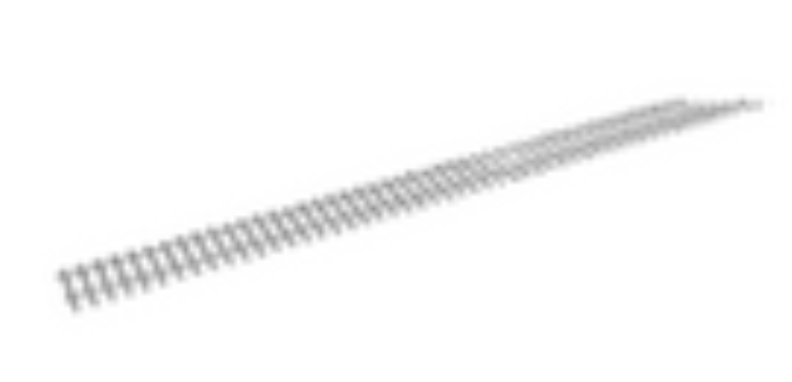
\includegraphics[width=4cm, height=3cm, keepaspectratio]{figures/rails.png}\\
\hline
Bridge & 2 & 0 & 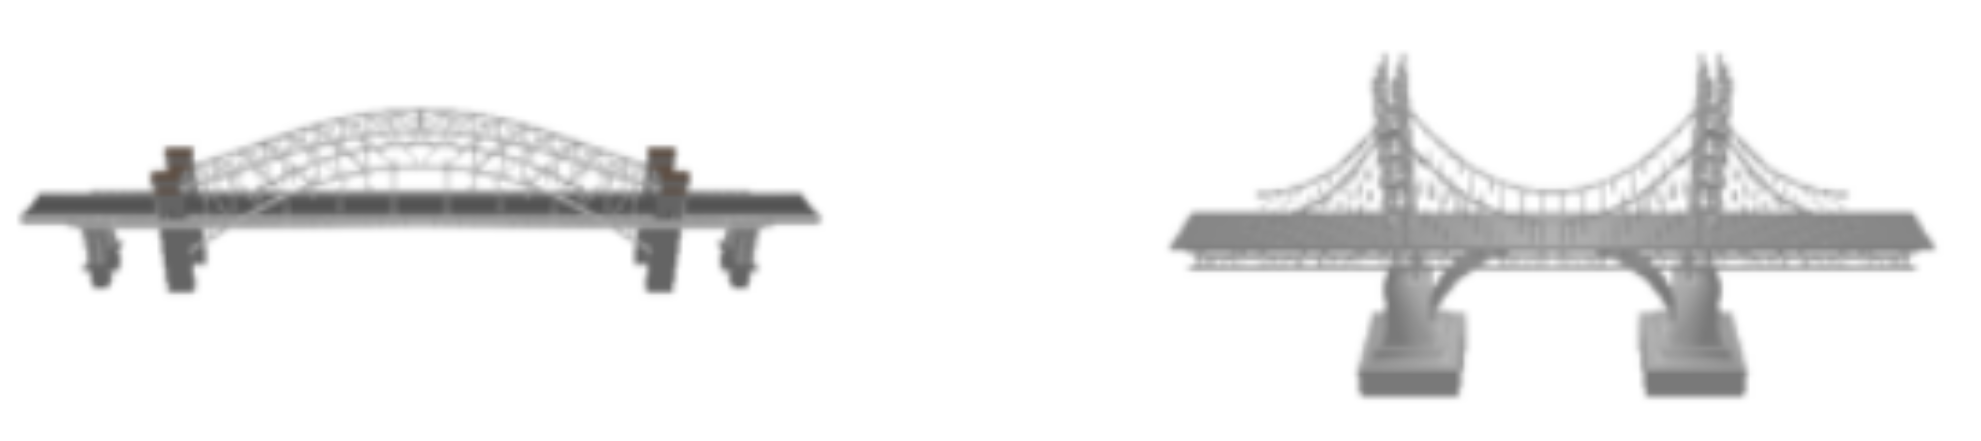
\includegraphics[width=4cm, height=3cm, keepaspectratio]{figures/bridges.png}\\
\hline
\end{tabular}

\end{table}

  
  
  \subsection{Accuracy}
  The accuracy proved to be very high, as on 22 runs with a batch size of 3, only 2 were incorrect. The incorrect ones were rerun and simply changing the batch size to 4 solved the issue. The issue is also primarily a rendering issue because these incorrect runs were using models that were untextured hence making it harder for CLIP to make accurate predictions. Surprisingly, it also worked very well with big 3D models such as bridges and railways. See table 2 for more detail.
  
\begin{table}[H]
\label{fig:accuracy}
\caption{Overview of runtime and accuracy}
\centering
\begin{tabular}{|c|c|c|c|c}
\hline
\textbf{Class} & \textbf{Average Render Time (s)} & \textbf{Average CLIP Time (s)} &  \textbf{Accuracy}\\
\hline
Car & 3.86 & 43.6 & 80\% \\
\hline
Helicopter & 61.85 & 38.87 & 100\%\\
\hline
Plane & 45.99 & 38.56 & 100\%\\
\hline
Train & 153.77 & 39.79 & 80\%\\
\hline
Railroad & 0.733 & 25.76 & 100\% \\
\hline
Bridge & 330.07 & 26.24 & 100\%\\
\hline
\end{tabular}

\end{table}
  
  \subsection{Importance of rendering}
  CLIP has already been very extensively tested in the original paper. It managed to achieve top-1 accuracy with accuracy of 85.4\%, which is comparable to state-of-the-art supervised models that were trained on massive amounts of labeled data. Hence, the weak link might be the rendering. The quality of the results depends heavily on the quality of the renders since CLIP was trained on real world data. Despite these limitations, we were able to accurately classify untextured or low polygon models just as well. It is hence necessary to find a sweet spot where the renders are good enough to give good results and at the same time be computationally cheap.
  
  \subsection{Runtime}
  As for the runtimes of the runs, the numbers may appear too big for the CLIP time. That is mainly due to the fact that we used the CPU for the runs, the performance on a GPU would naturally be faster. In average it takes 13 seconds for one traversal of the ontology, this number depends heavily on the depth of the ontology but does not depend on the image size (figure \ref{fig:fig1}). The more levels the ontology has, the more individual runs of CLIP are needed to reach a leaf class. This number is hence simply multiplied by the batch size to get the total time it takes for CLIP to traverse the ontology for all the images. See table 2 for more detail.
  \begin{figure}[h]
  	\centering
  	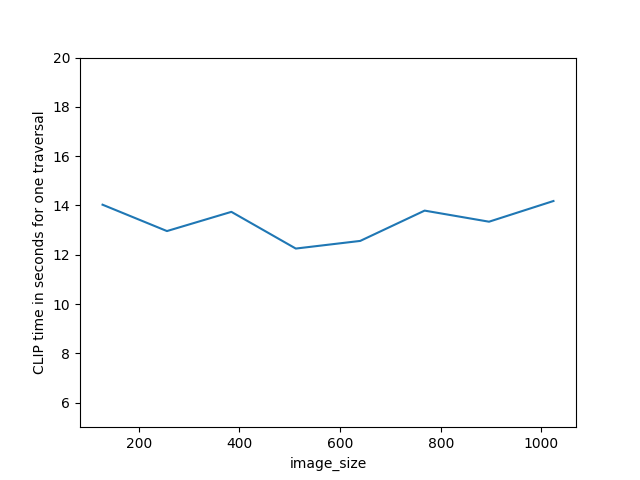
\includegraphics[width=0.6\textwidth]{figures/fig1.png}
  	\caption{CLIP runtime is independent of image size}
  	\label{fig:fig1}
  \end{figure}
  
  As for the rendering time, it mainly depends on the size of the 3D models, the batch size and the image size, the bigger one of these gets, the more time is needed to render the images. This makes sense because the renderer would need to render more pixels for the image size, and the more complicated the object is in terms of polygons, the more operations are needed to rasterize the model and calculate the appropriate lighting and so on (see figure \ref{fig:fig2}), and the bigger the batch size, the more images the renderer has to render. \\ \\
  As for the batch predictions runtime, it heavily depends on the batch size as well as the size of the ontology. The bigger the batch size the more time is needed. This is because CLIP traverses the whole ontology for each image, hence multiplying the time it takes to traverse the ontology once by the batch size (see figure \ref{fig:fig3}). \\ \\
  To summarize, the major influences on runtime are the following:
  \begin{itemize}
  \item \textbf{ontology depth}: increases the time needed for CLIP to traverse the ontology.
  \item \textbf{image size}: increases the time needed for rendering.
  \item \textbf{number of polygons}: increases the time needed for rendering.
  \item \textbf{batch size}: increases the time needed for rendering and the time needed for running CLIP on the ontology.
  \end{itemize}
  \begin{figure}[h]
  	\centering
  	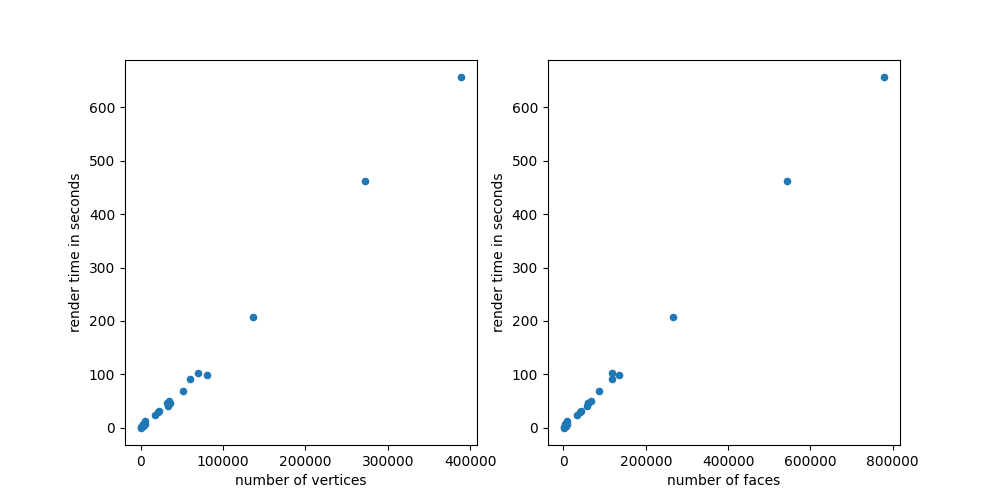
\includegraphics[width=\textwidth]{figures/two_plots.png}
  	\caption{Render time increases with 3D object size}
  	\label{fig:fig2}
  \end{figure} 
  \begin{figure}[H]
  	\centering
  	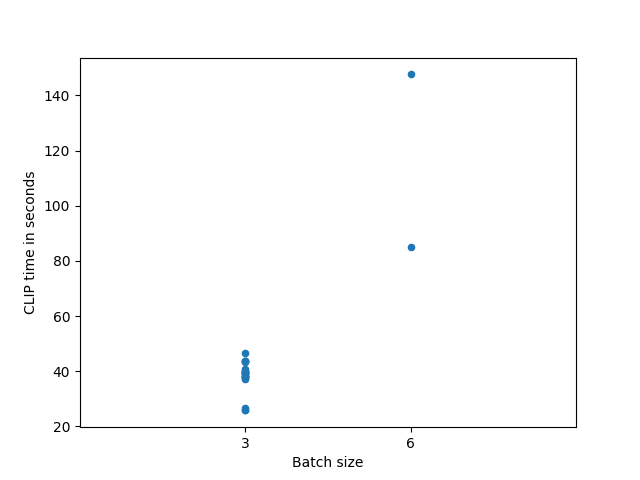
\includegraphics[width=0.6\textwidth]{figures/CLIP_time_batch.png}
  	\caption{CLIP time increases with batch size}
  	\label{fig:fig3}
  \end{figure} 
  
  \section{Discussion}
  \subsection{Key Finding}
  \subsubsection{Exploiting the ontology structure}
  A key achievement of this thesis is the ability of the process to exploit the tree-like structure of the ontology. By following one path in the tree, the process removes the need to explore every path. The semantic meaning of classes and subclasses allows the process to follow a certain heuristic that leads it to the correct class, for example, if CLIP sees a car, the it will be more likely to select vehicle rather than animal or transport infrastructure, hence totally disregarding the other paths. This of course then calls for the need to give the classes names that are expressive of the subclasses that follow.
  \subsubsection{Streamlined process}
  Another achievement is due to the excellent zero-shot capabilities of CLIP. The process can work with any ontology, given that the classes are expressively named, since CLIP relies heavily on the textual input. This also makes it very simple to add new classes to the ontology without the need of expanding the training dataset and further training. This means that the process can adapt to accurately classify classes of 3D models it has never seen before. Hence making it a zero-shot ontology-based classification algorithm.
  \subsubsection{Prompt engineering}
  Prompt engineering proved to be very useful when it comes to classifying with CLIP. This allows for innovative ways of using this concept, just like how we used it for classifying data properties in the ontology, we used the real meaning of the data property to prompt CLIP using sentences in natural language for determining the color of car, thus making the link between human and machine less abstract and more direct. 
  \subsection{Practical Implications}
  The most relevant practical implication comes from fact that using our method requires no extra training. This is a major advantage that decreases the time needed to integrate 3D models into digital twin assets ontologies in real world scenarios. 
  \subsection{Relations to previous research} 
  While the previous research mentioned in the literature review mainly used supervised models that use a specific set of classes, see research mentioned in 2.3. The process we used is unlimited in terms of possible classes and requires no further training. Another key difference is that our process can adapt to any kind of 3D models as long as it can be rendered as an image, previous research used descriptors that were specific to one kind of 3D model. Another difference is our reliance on the ontology structure to classify the 3D models, other research did not use ontologies very extensively. Our process could add to \cite{objectdetectionDT} to  further extend the data twin with 3D data from other sources.
  \subsection{Unexpected results and learned lessons}
  The most valuable lesson was the fact that we could adapt a model that was only supposed to work with images and adapted it to 3D models, sometimes it is better to use a pre-trained model and adapt it to our purposes instead of re-inventing the wheel. Another unexpected result how well CLIP was able to classify untextured models, as long as the outline of the object was good enough, CLIP could correctly classify the object. This is perhaps due to the fact that the CLIP training data also contained sketches. 
 
  \subsection{Limitations}
  \subsubsection{Object detection}
  One of the limitations of the process is the fact that it does not work very well when there are two or more objects on the scene, so it is currently a solution that only handles 3D models / scenes that only contain a single object to be classified. Furthermore, it does not perform object detection / segmentation but only simple classification.
  \subsubsection{Rendering}
  As mentioned in the results, the rendering plays a big role in the accuracy. It is hence essential to use good rendering and over all quality 3D models that are properly textured.
  \subsubsection{Slow runtimes}
  The process does not scale very well to bigger ontologies when it comes to CLIP predictions. It can also be very slow with bigger 3D models that need more time to render. 
  \subsection{Future research}
  Future research could address some of the limitations that we encountered. Most notably, the rendering part. Perhaps improved rendering or integration into 3D rendering software could make the whole process better and solve the rendering issues we encountered. Another point that future research could address is how to make the process able to perform image segmentation in order to classify more than one 3D model in the image. Additionally, the process could then also figure out the relationships between the two objects based on a relationship defined in the ontology.
  
  \section{Conclusions}
Through this thesis, we were able to answer the main research question "How can 3D objects be integrated into the digital asset ontology of transport infrastructure?" by using CLIP along with multi-view rendering of 3D models to accurately classify and the integrate the object by creating an instance for it in the ontology. We opted for mutli-view rendering since it allowed us to use existing multimodal model CLIP that usually only works with 2D images and make it work with 3D models. The excellent zero-shot capabilities of CLIP allowed the process to be very generalizable to any ontology with any digital twin assets hence not requiring the need for further training. While some limitations were met, like the fact that we the process does not support object detection, future investigations may look into how it would be possible to perform some sort of zero-shot image segmentation using the ontology classes. Additionally, the rendering we used was very basic and integrating the process into 3D editing software like Blender would have made things a lot faster. Furthermore, batch predictions proved to be very expensive to run in some cases, especially with bigger batch sizes, hence further emphasizing the need for better rendering in order to use smaller batch sizes.


  \newpage
  \bibliographystyle{IEEEtran}
  \bibliography{IEEEabrv, ./bsc-sample}
  %\printbibliography

\end{document}
